\chapter{Subgroups}
\label{ch:subgroups}


\section{Brief overview of the chapter}
\label{sec:subgp-overview}

TBW (and stolen from the below)

\section{Subgroups}
\label{sec:subgroups}
In our discussion of the group $\ZZ\defequi\Aut_{S^1}(\base)$ of integers in \cref{cha:circle} we discovered that some of the symmetries of $\base$ were picked out by the $n$-fold covering (for some particular natural number $n$).  On the level of the set $\base\eqto{}\base$, the symmetries picked out are all the iterates (positive or negative or even zero-fold) of $\Sloop^n$.  The important thing is that we can compose or invert any of the iterates of $\Sloop^n$ and get new symmetries of the same sort (because of distributivity $nm_1+nm_2=n(m_1+m_2)$).  So, while we do not get all symmetries of $\base$ (unless $n=1$), we get what we'd like to call a subgroup of the group of integers. 

% the ``subsymmetries'' formed a very organized structure.
% For each natural number $n$ we obtained a set of subsymmetries in the identity type $\base=\base$, namely the set of all the iterates $(\Sloop^{n})^m$ where $m$ varies over the integers.
% When $n$ was positive this was realized as the $n$-fold \covering of $S^1$, when $n=0$ this was given by the universal \covering.


The other extreme of the idea of a subgroup was exposed in \cref{sec:groupssubperm} in the form of the slogan ``any symmetry is a symmetry in $\Set$''.
By this we meant that, if $G \defequi \Aut_A(a)$ is a group, we produced a monomorphism $\rho_G:\Hom(G,\Aut_{\USymG}(\Set))$,
\ie any symmetry of $a$ is uniquely given by a symmetry (``permutation'') of the set $\USymG\defequi (a\eqto{}a)$.

For yet another example, consider the cyclic group $\CG_6$ of order $6$; perhaps visualized as the rotational symmetries of a regular hexagon,  \ie the rotations by $2\pi\cdot m /6$, where $m=0,1,2,3,4,5$.
The symmetries of the regular triangle (rotations by $2\pi\cdot m/3$, where $m=0,1,2$) can also be viewed as symmetries of the hexagon.
Thus there is a subgroup of $\CG_6$ which, as a group, is isomorphic to $\CG_3$.\marginnote{Make a TikZ drawing of the hexagon and triangle inscribe in it.}
There are other subgroups of $\CG_6$, and in this example they are accounted for simply by the various factorizations of the number $6$.

For other groups the subgroups form more involved structures and reveal much about the nature of the object whose symmetries we study.
There are several ways to pin down the subgroups and so capture this information.
If $A$ is a groupoid, singling out a group of subsymmetries of $a:A$ should be a way of picking out just some of the symmetries of $a$ in $A$ in a way so that we can compose subsymmetries compatibly.  To make a long story short; we want a group $H$ and a homomorphism $i:\Hom(H,G)$ so that $\USymi:\USymH\to\USymG$ is injective.\footnote{In classical set theory there is an important difference between saying that a function is the inclusion of a subset (which is what one classically wants) and saying that it is an injection.  We'll address this in a moment, so rest assured that all is well as you read on.}  We have a name for such a setup: $i$ is a \emph{monomorphism} as laid out in different interpretations in \cref{lem:eq-mono-cover}.

\subsection{Subgroups as monomorphisms}

The proposition $\ismono(i)$ is equivalent to saying that $\USymi:\USymH\to \USymG$ is an injection (all preimages of $\USymi$ are propositions), and also to saying that $\Bi:\BH\to\BG$ is a \covering, which in turn is equivalent to the proposition $\isset((\Bi)^{-1}(\shape_G))$ since $\BG$ is connected.
%\newcommand{\typemono}{Mono}
\begin{definition}
  \label{def:typeofmono}
  If $G$ is a group, the \emph{type of monomorphisms into $G$}\index{type! of monomorphisms into a groups}\glossary(MonoG){$\protect{\typemono_G}$}{type of monomorphisms into the group $G$} is
  $$\typemono_G\defequi\sum_{H:\typegroup}\sum_{i:\Hom(H,G)}\ismono(i)$$
  and the \emph{type of epimorphisms from $G$}\index{type! of epimorphisms from a groups}\glossary(EpiG){$\protect{\typeepi_G}$}{type of epimorphisms from the group $G$} is
  $$\typeepi_G\defequi\sum_{H:\typegroup}\sum_{f:\Hom(G,G')}\isepi(f).$$
  A monomorphism $(H,i,!)$ is
      \begin{enumerate}
      \item \emph{trivial}\index{trivial monomorphism} if $H$ is the trivial group, %.contractible (or, equivalently, if $\USym H$ is contractible),
      \item \emph{proper}\index{proper monomorphism} if $i$ is not an isomorphism.\qedhere
      \end{enumerate}
    \end{definition}
    \begin{exercise}
      \begin{enumerate}
      \item Show that $i:\Hom(H,G)$ is a monomorphism if and only if $Ui$ is an injection of sets and that $i$ is proper if and only $Ui$ is not a bijection.
      \item Show that $f:\Hom(G,G')$ is a monomorphism if and only if $Uf$ is an surjection of sets.
      \item Consider a composite $f=f_0f_2$ of homomorphisms.  Show that $f_0$ is an epimorphism if $f$ is and $f_2$ is a monomorphism if $f$ is.\qedhere
      \end{enumerate}
    \end{exercise}

\begin{example}
  \label{ex:sigma2inSigma3}
   \marginnote{
     That $i:\Sigma_2\to\Sigma_3$ is a monomorphism can visualized as follows: if $\Sigma_3$ represent all symmetries of an equilateral triangle in the plane (with vertices $1$, $2$, $3$), then $i$ is represented by the inclusion of the symmetries leaving $3$ fixed; \ie reflection through the line marked with dots in the picture.
   \[
     \begin{tikzpicture}[scale=1.5]
       \path (0:0)  node (one)   {$1$}
             (0:2)  node (two)   {$2$}
             (60:2) node (three) {$3$};
       \draw (one) -- (two);
       \draw (two) -- (three);
       \draw (three) -- (one);
       \draw[dotted] (three) -- (0:1);
     \end{tikzpicture}
   \]}
Consider the  homomorphism $i:\Sigma_2\to\Sigma_3$ of permutation groups corresponding to sending $A:\BSG_2\defequi \FinSet_2$ to $A+\bn1:\BSG_3$.
%This is a monomorphism since $\US i:\USym\Sigma_2\to\USym\Sigma_3$ is an injection.
\end{example}

\begin{example}
  \label{ex:prodinclismono}
  If $G_1$ and $G_2$ are groups, then the first projection from $G_1\times G_2$ is an epimorphism and the first inclusion into $G_1\times G_2$ is a monomorphism because their composite is the identity.
  % More generally, if $i:\Hom(H,G)$ is a homomorphism for which there (merely) exists a homomorphism $f:\Hom(G,H)$ such that $\id_H=fi$, then $i$ is a monomorphism.
  \end{example}

We will be interested in knowing when two monomorphisms into $G$ are identical.

\begin{lemma}
  \label{lem:setofsubgroups}
  Let $G$ be a group and $(H,i_H,!),(H',i_{H'},!):\typemono_G$ be two monomorphisms into $G$.  The identity type $(H,i_H,!)\eqto{}(H',i_{H'},!)$ is equivalent to
  \marginnote{
    \[
      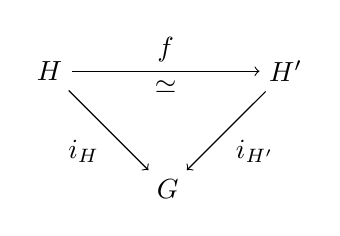
\begin{tikzpicture}[scale=1.5]
        \path (-1,0) node (H)  {$H$}
              (1,0)  node (H') {$H'$}
              (0,-1) node (G)  {$G$};
        \draw[->] (H) -- node[above] {$f$} node[below] {$\simeq$} (H');
        \draw[->] (H) -- node[below left] {$i_H$} (G);
        \draw[->] (H') -- node[below right] {$i_{H'}$} (G);
      \end{tikzpicture}
    \]
  }
  $$\sum_{f:\Hom(H,H')}\isEq(\US f)\times (i_{H'}\eqto{}i_H f)$$ and is a proposition.
  In particular, the type $\typemono_G$ of monomorphisms into $G$ is a set.
\end{lemma}
\marginnote{If you're familiar with the set-theoretic flavor of things, you know that it is important to distinguish between subgroups and injective group homomorphisms.
Our use of monomorphisms can be defended because two monomorphisms into $G$ are identical exactly if they differ by precomposition by an identitification.
In set-theoretic language this corresponds to saying that a subgroup is an injective abstract homomorphism \emph{modulo} the relation forcing that precomposing with an isomorphism yields identical subgroups.
Classical set-theory offers the luxury of having a preferred representative in every equivalence class: namely the image of the injection, type theory does not.  We only know that the type $\typemono$ is a set.}
\begin{proof}
By \cref{lem:isEq-pair=} an identity between $(H,i_H,!)$ and $(H',i_{H'},!)$ is uniquely given by an identity $p:H'\eqto{}_{\typegroup}H$ such that $i_{H'}\eqto{}i_H\,p$ (a proposition since $\Hom(H',G)$ is a set).
The description of the identity type follows since by univalence and \cref{cor:fib-vs-path}\ref{conn-fib-vs-path}, %\cref{lem:eqofconntypes},
the identity type $H\eqto{}H'$ is equivalent to the set
$$\sum_{f:\Hom(H,H')}\isEq(\US f).$$
% If $(H,i_H,!)$ is a subgroup of $G$, then

Now, $i_{H'}\eqto{}i_Hf$ is equivalent to $\US i_{H'}\eqto{}\US i_H \US f$, and since $\US i_H$ is an injection of sets there is at most one such function $\US f$; translating back we see that there is at most one $f$, making $\sum_{f%:\Hom(H,H')
}\isEq(\US f)\times (i_{H'}\eqto{}i_H f)$ a proposition.
% Consequently, the identity type
% $(H,i_H,!)\eqto{}_{\typesubgroup_G}(H,i_H,!)$ is equivalent to the type of homomorphisms $f:\Hom(H,H)$ which are such that $!:i_H^==i_H^=f^=$ and such that $f^=$ is an equivalence (as we see in a moment this last requirement is redundant).
% Now, since $(H,i_H,!)$ is a subgroup, $i_H^=$ is an injection of sets, which forces $!:f^==\refl{\USym H}$, which ultimately forces $f$ to be (identical to) the identity homomorphism.
\end{proof}

\subsection{Subgroups through $G$-sets}

For many purposes it is useful to define ``subgroups'' slightly differently.
A monomorphism into $G$ is given by a pointed connected groupoid  $\BH=(\BH_\div,\pt_H)$, a function $F:\BH_\div\to\BG_\div$ whose fibers are sets (a \covering) and an identification $p_f:\shape_G\eqto{}F(\shape_H)$.  There is really no need to specify that $\BH_\div$ is a groupoid: if $F:T\to \BG$ is a \covering, then $T$ is automatically a groupoid.

On the other hand,  the type of \coverings over $\BG$ is equivalent to the type of $G$-sets: if $X:\BG\to\Set$ is a $G$-set, then the \covering is given by the first projection $\tilde X\to \BG$ where $\tilde X\defequi\sum_{y:\BG}X(y)$ and the inverse is obtained by considering the fibers of a \covering.  Furthermore, we saw in \cref{lem:conistrans} that $\tilde X$ being connected is equivalent to the condition $\istrans(X)$ of \cref{def:transitiveGset} claiming that the $G$-set $X$ is transitive.

Hence, the type (set, really) $\typemono_G$ of monomorphisms into $G$ is equivalent to the type of pointed connected \coverings over $\BG$, which again is equivalent to the type $\typesubgroup_G$ of transitive $G$-sets $X:\BG\to\Set$ together with a point in $X(\shape_G)$.

\begin{definition}\label{def:set-of-subgroups}
  Let $G$ be a group then the set of \emph{subgroups of $G$}\index{type!of subgroups of a group}\glossary(SubG){$\protect{\typesubgroup_G}$}{type of subgroups of $G$} is
  $$\typesubgroup_G\defequi\sum_{X:\BG\to\Set}{\,}X(\shape_G)\times\mathrm{isTrans}(X).$$
  The preferred equivalence
  with the set of monomorphisms into $G$ is given by the function
  \marginnote{%
   The inverse equivalence to $E$ is given by sending $(X,\pt,!)$ to the monomorphism associated with the first projection $\sum_{z:\BG}X(z)\to\BG$.
 }%
 $$E:\typemono_G\to\typesubgroup_G\qquad (H,i,!)\mapsto E(H,i,!)\defequi ((Bi)^{-1},(\shape_H,p_i),!),$$
 %\glossary(E){$E$}{equivalence from $\typemono_G$ to $\typesubgroup_G$}
  where the monomorphism $i:\Hom(H,G)$ is -- as always -- given by the pointed map $(Bi_\div,p_i):(\BH_\div,\shape_H)\to_*(\BG_\div,\shape_G)$; and where the preimage $(Bi)^{-1}:\BG\to\Set$ is a $G$-\emph{set} since $i$ is a monomorphism  and finally $(\shape_H,p_i):(Bi)^{-1}(\shape_G)\defequi \sum_{x:\BH}(\shape_G\eqto{}Bi(x))$.
\end{definition}

\marginnote{%
  Which of the equivalent sets $\typemono_G$ and $\typesubgroup_G$ is allowed to be called ``the set of subgroups of $G$'' is, of course, a choice.  It could easily have been the other way around and we informally refer to elements in either sets as ``subgroups'' and use the given equivalence $E$ as needed.
}%
\marginnote{%
  An argument for our choice can be
  as follows.  In set-based mathematics one has two options for defining subgroup: either as a certain subset (uniquely given by its characteristic function to $\Prop$) or as an equivalence class of injections (taking care of size issues since the class of monomorphisms will not form a small set).  The former is the usual choice and is the one we model here with $\typesubgroup_G$, whereas the other corresponds to $\typemono_G$
  % that the identity type in $\typesubgroup_G$ seems more transparent than the one in $\typemono_G$  (``more things are equal'' in $\typemono_G$?), just as  $A\to\Prop$ gives more the intuition of picking out a subset by means of a characteristic function than what you get when considering the equivalent type of injections into $A$.
}
  \begin{example}
    The monomorphism of $\Sigma_2$ into $\Sigma_3$ of \cref{ex:sigma2inSigma3} can be displayed as a subgroup of $\Sigma_3$ through
    $$X:\FinSet_3\to\Set
    $$
    given by $A\mapsto\sum_{B:\FinSet 2}(A\eqto{}B+\bn 1)$ together with a proof that this is a set; in fact, the identity type $(B,p)\eqto{}(B',p')$ is equivalent to $\sum_{q:B\eqto{}B'}(q+\bn 1)p\eqto{}p'$ which is a proposition since $q$ is uniquely given by $q+\bn 1\eqto{}p'p^{-1}$.
  \end{example}
  \begin{xca}
    Given a group $G$ we defined in \cref{sec:groupssubperm} a monomorphism from $G$ to the permutation group $\Aut_{\USym G}(\Set)$. Write out the corresponding subgroup of $\Aut_{\USym G}(\Set)$.
  \end{xca}
\begin{example}
  \label{ex:prodinclisGset}
  We saw in \cref{ex:prodinclismono} that the first inclusion $i_1:G\to G\times G'$ is a monomorphism.
  The corresponding $G\times G'$-set is the composite of the first projection $\mathrm{proj}_1:\BG_\div\times\BG'_\div\to \BG_\div$ followed by the principal $G$-torsor $\princ G:\BG\to\Set$.

  More generally, if $i:\Hom(H,G)$ and $f:\Hom(G,H)$, and $fi\eqto{}\id_H$, then $(H,i,!):\typemono_G$, corresponding to the subgroup with $G$-set given by the composite of $\Bf$ with the princial $H$-torsor $\princ H$.
\end{example}



  Translating the concepts in \cref{def:typeofmono} through the equivalence $E$ we say that a subgroup $(X,\pt,!):\typesubgroup_G$ is
      \begin{enumerate}
      \item \emph{trivial}\index{trivial subgroup} if $X$ is identical to the principal $G$-torsor.
      \item \emph{proper}\index{proper subgroup} if $X(\shape_G)$ is not contractible.
      \end{enumerate}

      \begin{remark}
      \label{rem:notationsubgroup}
      A note on classical notation is in order.
If $(X,\pt,!)$ is a subgroup corresponding to a monomorphism $(H,i,!)$ into a group $G$, tradition would permit us to relax the burden of notation and we could write ``a subgroup $i:H\subseteq G$'', or, if we didn't need the name of $i:\Hom(H,G)$, simply ``a subgroup $H\subseteq G$'' or ``a subgroup $H$ of $G$''.
    \end{remark}

    % commented out by BID 211117 Some examples and references should be included when the cyclic subgroups are fully developed
    % \subsection{The geometry of subgroups: some small examples}\footnote{this subsection is not touched: it needs attention}
% \label{smallsubgpex}

% As a teaser, and in order to get a geometric feel for the subgroups and their intricate interplay, it can be useful to have some fairly manageable examples to stare at.
% Some of the main tools for analyzing the geometry of subgroups are collected in \cref{sec:fingp} on finite groups, and we hope the reader will be intrigued by our mysterious claims and go on to study \cref{sec:fingp}.
% That said, the examples we'll present are possible to muddle through by hand without any fancy machinery, but brute force is generally not an option and even for the present examples it is not something you want to show publicly.

% When presenting the subgroups of a group $G$, three types are especially revealing: the set of subgroups $\typesubgroup_G(\shape_G)$, the \emph{groupoid of subgroups} $\typesubgroup(G)\defequi\sum_{y:\BG}\typesubgroup_G(y)$ and what we for now call the ``set of normal subgroups'' $\prod_{y:\BG}\typesubgroup_G(y)$.   Our local use of ``normal subgroup'' is equivalent to the official definition to come.

% The first projection $\typesubgroup(G)\to \BG$ is referred to as the \emph{\covering of subgroups}.

% \footnote{Write out and fix the concrete examples (cyclic groups and $\Sigma_3$) commented out}
% % \begin{remark}
% % In  \cref{cha:circle} we studied the subgroups of the group of integers $G\eqto{}\ZZ$ through \coverings over the circle $S^1$ (which we showed was equivalent to $B\ZZ$).
% % We discovered a subgroup $n\ZZ$ for each natural number $n:\NN$ and in the groupoid $\typesubgroup({\ZZ})$ these sit as elements in separate components.  Each of these components are contractible (because addition is commutative: $\ZZ$ is an abelian group).

% % In general, a component $K$ of the groupoid $\sum_{y:\BG}\typesubgroup_G(y)$ of subgroups of a group $G$ may be much more interesting. For one thing the, $K$ can contain many subgroups in the sense that the preimage of the first projection $K\to \BG$ is a set that may have many different elements; each representing a subgroup.  However, this set of subgroup will be a \emph{conjugacy class} of subgroups: the different subgroups are related by the conjugation action of $G$.

% % If $G$ is abelian this action is trivial, and $\sum_{y:\BG}\typesubgroup_G(y)$ consists of contractible components indexed over the subgroups of $G$.  Otherwise different subgroups may live in the same component of the groupoid of subgroups -- we'll see examples in a moment.

% % In addition, the components will not in general be contractible, revealing the symmetries of the subgroups under the conjugation action.
% % \end{remark}


% % \begin{example}
% %   The trivial group only has itself as a subgroup; the groupoid of subgroups and the set of normal subgroups are singletons.
% % \end{example}
% % \begin{example}
% %   The cyclic group $C_p$ of prime order $p$ has only two subgroups, the trivial and the full subgroup itself and both are normal.  In fact, all subgroups of abelian groups are normal.

% % In general, the cyclic group $C_n$ of order $n$ has exactly one subgroup for each divisor $i$ of $n$.
% % \end{example}


% % \begin{example}
% %   The group $C_2\times C_2$ has has no less than five subgroups: the trivial one, three subgroups that as groups (as opposed as \emph{sub}groups) are equivalent to $C_2$ and the full group $C_4$ itself.
% % \end{example}
% % \begin{remark}
% %   The permutation group $\Sigma_3$ has four nontrivial proper subgroups.  Three conjugate subgroups isomorphic as groups to $C_2$ and one normal one which is as a group is isomorphic to $C_3$.  The component containing the copies of $C_2$ is equivalent to a circle.
% % \end{remark}
\section{Images, kernels and cokernels}
\label{subsec:ker}

The set of subgroups of a group $G$ encodes much information about $G$, partially because homomorphisms between $G$ and other groups give rise to subgroups.

In \cref{ex:Cm} we studied a homomorphism from $\ZZ$ to $\Sigma_m$ defined via the pointed map $R_m:S^1\to_*\BSG_m$ given by sending $\base$ to $\bn m$ and
$\Sloop$ to the cyclic permutation $s_m\colon\USym\Sigma_m\oldequiv(\bn m\eqto{}\bn m)$, singling out the iterates of $s_m$ among all permutations.  From this we defined the group $C_m$ through a quite general process which we define in this section, namely by taking the \emph{image} of $R_m$.

We also noted that the resulting pointed map from $S^1$ to $\B C_m$ was intimately tied up with the $m$-fold \covering $-^m:S^1\to_*S^1$ -- picking out exactly the iterates of $\Sloop^m$ -- which in our current language corresponds to a monomorphism $i_m:\Hom(\ZZ,\ZZ)$. This process is also a special case of something, namely the \emph{kernel}.

The relations between the cyclic groups in the forms $\ZZ/m$, $C_m$ and $C'_m$ as in \cref{ex:cyclicgroups} are also special cases of  what we do in this section.

\marginnote{For those familiar with the classical notion, the following summary may guide the intuition.}

 \marginnote{ If $\phi:\Hom^\abstr(\mathcal G,\mathcal G')$ is an abstract group homomorphism, the preimage $\phi^{-1}(e_G)$ is an abstract subgroup which is classically called the kernel of $\phi$.}

\marginnote{On the other hand, the cokernel is the quotient set of $\mathcal G'$ by the equivalence relation generated by  $g'\sim g'\cdot\phi(g)$ whenever $g:\mathcal G$ and $g':\mathcal G'$.}

In our setup with a group homomorphism
$f:\Hom(G,G')$ being given by a pointed function $\Bf:\BG\to_*\BG'$, the above mentioned kernel, cokernel and image are just different aspects of the preimages
$$(\Bf)^{-1}(z)\defequi\sum_{x:\BG}(z\eqto{}\Bf(x))$$
for $z:\BG'$.  Note that all these preimages are groupoids.

The kernel will correspond to a preferred component of the preimage of $\shape_{G'}$, the cokernel will be the ($G'$-)set of components and for the image we will choose the monomorphism into $G'$ corresponding to the cokernel.  This point of view makes it clear that the image will be a subgroup of $G'$, the kernel will be a subgroup of $G$, whereas there is no particular reason for the cokernel to be more than a ($G'$-) set.
\marginnote{Even though the cokernel is in general just a $G'$-set, we will see in \cref{def:normalquotient} that in certain situations it gives rise to a group called the quotient group. }

\subsection{Kernels and cokernels}
The kernel of $f\colon\Hom(G,G')$ is a component of the fiber of $\Bf$, whereas the cokernel is the set of components of the fiber.  We spell out the details.
\label{sec:kerandcoker}
\begin{definition}
  \label{def:kernel}
 We define a function
  $$\ker:\Hom(G,G')\to\typemono_G$$
  which we call the \emph{kernel}\index{kernel}.
  If $f:\Hom(G,G')$  is a homomorphism we must specify the ingredients in  $\ker f\defequi(\Ker f,\incl_{\ker f},!):\typemono_G$.
  The classifying $\B\Ker f$ space of the \emph{kernel group}\index{kernel!group}
  %\glossary(Ker f){$\protect{\Ker f}$}{the kernel group of the homomorphism $f$}
\marginnote{There is an inherent abiguity in our notation:
  is the kernel of $f$ a group or a monomorphism into $G$?
  This is common usage and is only resolved by a typecheck.}
 (or most often just the ``kernel'') is the component of the fiber of $Bf$ pointed by
 $$\shape_{\Ker f}\defequi(\shape_G,p_f):(\Bf)^{-1}(\shape_{G'})$$
 \marginnote{that is $$\Ker f\defequi \Aut_{(\Bf)^{-1}(\shape_{G'})}(\shape_G,p_f)
$$} (where $p_f:\shape_{G'}\eqto{}\Bf(\shape_G)$ is the part of $\Bf$ claiming it is a pointed map).
The first projection $B\Ker f\to \BG$ is a \covering (by \cref{cor:contract-away} the preimages are equivalent to the sets $\sum_{p:\shape_{G'}\eqto{}\Bf(z)}\Trunc{\shape_{\Ker f}\eqto{}(z,p)}$) giving a monomorphism
% $\kermap f$
$\incl_{\ker f}$ of $\Ker f$ into $G$; together defining $\ker f\defequi(\Ker f,\incl_{\ker f},!):\typemono_G$.
\end{definition}

Written out, the classifying type of the kernel,
$B\ker f_\div$, is $$\sum_{z:\BG}\sum_{p:\shape_{G'}\eqto{}f(z)}\Trunc{(\shape_G,p_f)\eqto{}(z,p)}$$
and $\incl_{\ker f}:\Hom(\Ker f, G)$ is given by the first projection.

\begin{definition}
  \label{def:cokernel}
  Let $f:\Hom(G,G')$  be a homomorphism.
  The \emph{cokernel}\index{cokernel}%
  \glossary(coker){$\protect\coker f$}{cokernel of a homomorphism $f$}
  of $f$ is the $G'$-set
\[
  \coker f:\BG'\to\Set,\qquad \coker f(z)\defequi  \Trunc{(\Bf)^{-1}(z)}_0;
\]
defining a function of sets\marginnote{%
  The associated $\abstr(G')$-set $\coker f(\shape_{G'})$ is (also) referred to
  as the (abstract) cokernel of $f$.}
\[
  \coker:\Hom(G,G')\to G'\text{-}\Set.\qedhere
\]
\end{definition}

If a monomorphism $i$ from $G$ to $G'$ is clear from the context (``$G\subseteq G'$''), we may write $G'/G$ for the cokernel of $i$.
% \newcommand*{\kermap}[1]{\mathrm{in}_{\ker #1}} something wrong fix
\begin{lemma}
  \label{lem:coker is transitive}
  The cokernel $\coker f$ is a transitive $G'$-set.
  %solution: 
\end{lemma}
\begin{proof}
  It is enough to show that for all $|x,p|\in\coker(\shape_{G'})$ there is a $g:\UG$ s.t. $g\cdot |\shape_G,p_f|\eqto{} |x,p|$.  It suffices to do this for $x$ being $\shape_G$, and then $g\defequi p_f^{-1}p$ will do.
\end{proof}
\begin{remark}
  \label{remark:imageandcokernel}
\marginnote{The subgroup of $G'$ associated with the cokernel is the ``image'' of the next section.}
  Since the cokernel is a transitive $G'$-set, we need just to provide $\coker f(\shape_{G'})\defequi\Trunc{\Bf^{-1}(\shape_{G'})}_0$ with a point to say that the cokernel defines a subgroup of $G'$. The obvious point to choose is $|\shape_G,p_f|$. In the next section we will consider this subgroup in more detail and call it the image of $f$.

Another proof of $\coker f$ being a transitive $G'$-set would be to say that since $BG$ is connected and equivalent to $\sum_{z:\B G'}\Bf^{-1}(z)$ which maps surjectively onto $\sum_{z:\BG'}\Trunc{\Bf^{-1}(z)}_0$ the latter is connected -- and, when pointed at $(\shape_{G'},|\shape_G,p_f|)$, just another name for $E(\coker f):\typemono_{G'}$.
\end{remark}


\begin{xca}
  Given a homomorphism $f:\Hom(G,G')$, prove that
    \marginnote{Hint: consider the corresponding property of the preimage of $\Bf$.
    \[
      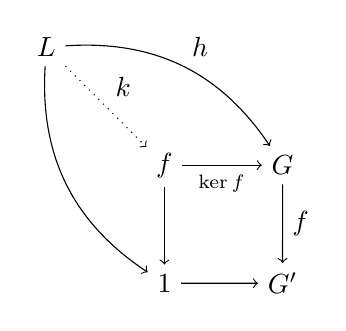
\begin{tikzpicture}[scale=1.5]
        \path (-1,1) node (L)   {$L$}
              (0,0)  node (Ker) {$\Ker f$}
              (1,0)  node (G)   {$G$}
              (0,-1) node (one) {$1$}
              (1,-1) node (G')  {$G'$};
        \draw[->,dotted] (L) -- node[above right] {$k$} (Ker);
        \draw[->] (L) to[bend left] node[above right] {$h$} (G);
        \draw[->] (L) to[bend right] (one);
        \draw[->] (Ker) -- node[below] {$\incl_{\ker f}$} (G);
        \draw[->] (Ker) -- (one);
        \draw[->] (G) -- node[right] {$f$} (G');
        \draw[->] (one) -- (G');
      \end{tikzpicture}
    \]
    }
  \begin{enumerate}
  \item $f$ is a monomorphism if and only if the kernel is trivial
  \item $f$ is an epimorphims if and only if the cokernel is contractible.
  \item if $h:\Hom(L,G)$ is a homomorphism such that $fh:\Hom(L,G')$ is the
    trivial homomorphism (equivalently, $fh$ factors through the trivial group $1$),
    then there is a unique $k:\Hom(L,\Ker f)$ such that
    $h\eqto{}\incl_{\ker f}k$.\qedhere
  \end{enumerate}
\end{xca}


The kernel, cokernel and image constructions satisfy a lot of important relations which we will review in a moment, but in our setup many of them are just complicated ways of interpreting the following fact about preimages (see the illustration\footnote{
  \[
    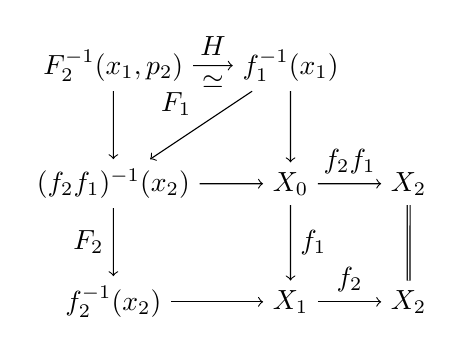
\begin{tikzpicture}[scale=1.5]
      \path (-.5,2) node (02)  {$F_2^{-1}(x_1,p_2)$}
            (1,2)   node (12)  {$f_1^{-1}(x_1)$}
            (-.5,1) node (01)  {$(f_2f_1)^{-1}(x_2)$}
            (1,1)   node (11)  {$X_0$}
            (2,1)   node (21)  {$X_2$}
            (-.5,0) node (00)  {$f_2^{-1}(x_2)$}
            (1,0)   node (10)  {$X_1$}
            (2,0)   node (20)  {$X_2$};
      \draw[->]
        (02) edge node[left]  {$\fst$} (01)
        (01) edge node[left]  {$F_2$}  (00)
        (12) edge node[right] {$\fst$} (11)
        (11) edge node[right] {$f_1$}  (10)
        (21) edge[-,double]            (20)
        (02) edge node[above] {$H$} node[below] {$\simeq$} (12)
        (01) edge node[above] {$\fst$} (11)
        (11) edge node[above] {$f_2f_1$} (21)
        (00) edge node[above] {$\fst$} (10)
        (10) edge node[above] {$f_2$} (20)
        (12) edge node[above left] {$F_1$} (01);
    \end{tikzpicture}
  \]
} in the margin  for an overview)
\begin{lemma}
  \label{lem:fibersofcomposites}
  Consider pointed functions $(f_1,p_1):(X_0,x_0)\to_*(X_1,x_1)$ and $(f_2,p_2):(X_1,x_1)\to_*(X_2,x_2)$ and the resulting functions
  $$F_1:f_1^{-1}(x_1)\to(f_2f_1)^{-1}(x_2),\qquad F_1(x,p)\defequi(x,p_2f_2p),$$
  $$F_2:(f_2f_1)^{-1}(x_2)\to f_2^{-1}(x_2),\qquad F_2(x,q)\defequi(f_1x,q)$$
  \marginnote{(here the function $\xymatrix{((x_1,p_2)\eqto{}(f_1x,q))\ar[r]^-{\pathpair p r\mapsto p}&(x_1\eqto{}f_1(x))}$ is the ``first projection'' explained in the discussion of the interpretation of pairs following \cref{def:pairtopath})}
  $$H:F_2^{-1}(x_1,p_2)%\oldequiv\sum_{(x,q)\in (f_2f_1)^{-1}(x_2)}((x_1,p_2)\eqto{}(f_1x,q))\to \\
  \to f_1^{-1}(x_1),\qquad H(x,q,\pathpair p r)\defequi (x,p))$$


Then
\begin{enumerate}
\item $H$ is an equivalence with inverse
$$H^{-1}(x,q)\defequi((x,p_2f_2(q)),(\overline{q,\refl{p_2f_2(q)}})),$$
\item the composite $F_1H$ is identical to the first projection
  $$\fst:{F_2^{-1}(x_1,p_2)\to(f_2f_1)^{-1}(x_2)},$$
  more precisely, if $(x,q,\pathpair p r):F_2^{-1}(x,p_2)$, then $\fst(x,q,\pathpair p r)$ is $(x,q)$, whereas $F_1H(x,q,\pathpair p r)$ is $(x,p_2f_2p)$ and $r:p_2f_2p\eqto{}q$ provides the desired element in $F_1H\eqto{}\fst$.
\end{enumerate}
\end{lemma}
\begin{proof}
  That $H$ is an equivalence is seen by noting that $F_2^{-1}(x_1,p_2)$ is equivalent to
  $\sum_{x:X_0}\sum_{q:x_2\eqto{}f_2f_1x}\sum_{p:x_1\eqto{}f_1x}q\eqto{}p_2f_2p$ and that $\sum_{q:x_2\eqto{}f_2f_1x}q\eqto{}p_2f_2p$ is contractible.
\end{proof}
% When referring to \cref{lem:fibersofcomposites}
% it is often useful to display an

Hence, through univalence, $H$ provides an identification
  $$\bar H:(F_2^{-1}(x_1,p_2),\fst)\eqto{}(f_1^{-1}(x_1),F_1)$$ in the type $\sum_{X:\UU}(X\to(f_2f_1)^{-1}(x_2))$ of function with codomain $(f_2f_1)^{-1}(x_2)$.
  % ($\fst(t)$ refers to the discussion following \cref{def:pairtopath} so that if $t\oldequiv(\overline{a,b}):(x_1,p_1)\eqto{}(x,p_1f_2q)$, then $\fst(t)\defequi a:x_1\eqto{}f_1x$).
  
From the universal property of the preimage it furthermore follows that $F$ is the unique map such that $\fst F\eqto{}_{f_1^{-1}(x_1)\to X_0}\fst$ and $H^{-1}$ is similarly unique with respect to $\fst H^{-1}\eqto{}F$.

\begin{corollary}
  \label{cor:cokermaps}
  \marginnote{$$\xymatrix{\Ker f_1\ar@{=}[r]\ar[d]^{F_1}&\Ker f_1\ar[d]^{\incl_{\ker f_1}}\\
      \Ker f_2f_1\ar[d]^{F_2}\ar[r]^-{\incl_{\ker f_2f_1}}&G_0\ar[d]^{f_1}\ar[r]^{f_2f_1}&G_2\ar@{=}[d]\\
      \Ker f_2\ar[r]^-{\incl_{\ker f_2}}&G_1\ar[r]^{f_2}&G_2% \\
   % \coker F_2&\coker f_1
 }
  $$}
  Consider two composable homomorphisms $f_1:\Hom(G_0,G_1)$ and $f_2:\Hom(G_1,G_2)$.
  There is a unique monomorphisms $F_1$ from $\Ker f_1$ to $\Ker(f_2f_1)$
  and a unique homomorphism $F_2$ from $\Ker(f_2f_1)$ to $\Ker f_2$ such that $\incl_{\ker f_1}\eqto{}\incl_{\ker f_2f_1}F_1$ and $f_1\incl_{\ker f_2f_1}\eqto{}\incl_{\ker f_2}F_2$.
  Furthermore, $$F_1\eqto{}_{\typemono_{G_1}}\incl_{\ker F_2}$$ and $$(\coker f_1)\,\B\incl_{\ker f_2}\eqto{}_{\B\Ker f_2\to\Set}\coker (F_2).$$

  Consequequently,
  \begin{enumerate}
  \item if $f_2$ is a monomorphism then $F_1:\Ker f_1\to\Ker f_2f_1$ is an isomorphism and
  \item if $f_1$ is a monomorphism then $F_2:\Ker f_2f_1\to\Ker f_2$ is an isomorphism.
  \end{enumerate}
\marginnote{If $f,g:A\to\Set$ are two $A$-sets, then $f\to g$ is defined to be the set $$\prod_{a:A}(f(a)\to g(a))$$ and we say that $\phi:f\to g$ is an equivalence if $\prod_{a:A}\isEq\phi(a)$; see \cref{lem:fiberwise}.}
Likewise, the set truncation of the maps $F_1$ and $F_2$ constructed in \cref{lem:fibersofcomposites} give maps  of families
$$F_1':\coker f_1\to_{\BG_1\to\Set}\coker(f_2f_1)\,Bf_2,\quad F_2':\coker(f_2f_1)\to_{\BG_2\to\Set}\coker f_2$$
  such that
  \begin{enumerate}
  \item if $f_2$ is an epimorphism then $F_1':\coker f_1\to_{\BG_2\to\Set}\coker(f_2f_1)\,Bf_2$ is an equivalence and
  \item if $f_1$ is an epimorphism then $F_2':\coker(f_2f_1)\to_{\BG_2\to\Set}\coker f_2$  is an equivalence.
  \end{enumerate}
\end{corollary}
\begin{xca}
  Let $f:\Hom(G,G')$.  Then the subgroup $E(\ker f):\typesubgroup_G$ associated with the kernel is given by a $G$-set equivalent to the one sending $x:\BG$ to
  $$\sum_{p:\shape_{G'}\eqto{}\Bf(x)}\Trunc{\sum_{\beta:\shape_G\eqto{}x}p\eqto{}\USym f(\beta)p_f}.$$
  If $f$ is an epimorphism this is furthermore equivalent to
  $$x\mapsto(\shape_{G'}\eqto{}\Bf(x)).$$
\end{xca}

\subsection{The image}
\label{sec:image}


For a function $f:A\to B$ of sets (or, more generally, of types) the notion of the ``image'' gives us a factorization through a surjection followed by an injection: noting that $a\mapsto (f(a),!)$ is a surjection from $A$ to the ``image'' $\sum_{b:B}\Trunc{f^{-1}(b)}$, from which we have an injection (first projection) to $B$.
\marginnote{The formula for the image in group theory is the same as the one for sets, except that the propositional truncation we have for the set factorization is replaced by the set truncation present in our formulation of the cokernel $\coker(f)\defequi\Trunc{(\Bf)^{-1}(z)}_0$.}
This factorization
$$A\to\sum_{b:B}\Trunc{f^{-1}(b)}\to B$$
is unique (\cref{xca:unique-fact-image}).

For a homomorphism $f:\Hom(G,G')$ of groups we similarly have a unique factorization
$$G\to \Img f \to G'
$$
through an epimorphism followed by a monomorphism which, on the level of connected groupoids, is given by
$$\xymatrix{
  {\BG_\div}\ar[rrr]^-{x\mapsto(\Bf(x),\trunc{(x, \refl {\Bf(x)})}_0)}&&&
  \sum_{z:{BG'_\div}}\Trunc{({\Bf})^{-1}(z)}_0\ar[rr]^-{\fst} &&{BG'_\div,}
}$$
together with base point information.
In particular, we choose the base point $(\shape_{G'},\trunc{(\shape_G,p_f)}_0)$, so that the \emph{image group} is  %type $\sum_{b:B}\Trunc{f^{-1}(b)}$ is simply replaces by
$$\Img f\defequi\Aut_{\sum_{z:\BG'}\Trunc{(\Bf)^{-1}(z)}_0}((\shape_{G'},\trunc{(\shape_G,p_f)}_0)).$$
In other words, the image is nothing but the subgroup of ${G'}$ associated with the cokernel as discussed in \cref{remark:imageandcokernel}.

\begin{xca}\label{xca:IMg_pointed}
With the choice of point of $\Img f$ above, give paths for
${x\mapsto(\Bf(x),\trunc{(x, \refl {\Bf(x)})}_0)}$ and ${\fst}$
so that these maps become pointed maps whose composition is indeed 
equal to the pointed map $\Bf$.
Show that these pointed maps indeed give an epimorphism and a monomorphism, respectively.
Hint: for the epimorphism, use \cref{lem:trunc-n-connected}.
\end{xca}

That the image gives a \emph{unique factorization} is elegantly expressed by saying that it is the unique inverse of composition.
We use the pullback construction from \cref{def:pullback} to express the type of epi/mono factorizations of homomorphisms from $G$ to $G'$ as $\typeepi_G\times_{\typegroup}\typemono_{G'}$ where the maps to $\typegroup$ are understood to be the first projections
(so that the epimorphisms and monomorphisms in question can, indeed, be composed).


  \begin{construction}\label{con:im}
    For all groups $G,$ and $G'$ the map
    $$
    \circ:\typeepi_G\times_{\typegroup}\typemono_{G'}\to\Hom(G,G')
    $$
    given by composition,\footnote{here $p$ is an epimorphism from $G$ to the group $Z$, $j$ a monomorphims from the group $Z'$ to $G'$, $\alpha\colon Z\eqto{}Z$
      and $\ptoe\alpha$ is the isomorphism corresponding to the identification $\alpha\colon Z\eqto{}Z'$, as in \cref{def:idtoeq},
      so that the composite looks like
    $$\xymatrix{G\ar[r]^p& Z\ar[r]^{\ptoe\alpha}_\sim&Z'\ar[r]^j&G'}$$}
    %\marginnote{$\xymatrix{G\ar[r]^p& Z\ar@{=}[r]^\alpha_\to&Z'\ar[r]^j&G'}$}
    $$\circ((Z,p,!),(Z',j,!),\alpha)\defequi j\ptoe \alpha p$$
    is an equivalence
    with inverse given by the image factorization.
\end{construction}
\begin{implementation}{con:im}
  For any integer $n\geq -1$ -- and in our case for $n=0$ -- on the level of types the factorization of a function $f\colon X\to Z$ as
  $$\xymatrix{X\ar[rrr]^-{x\mapsto (f(x),\trunc{(x,\refl{f(x)})}_n)}&&&\sum_{z:Z}\Trunc{f^{-1}(z)}_n\ar[rr]^\fst&&Z
  }$$
  is unique in the sense that
  \begin{quote}
    if $p:f\eqto{}jq$ where $q\colon X\to Y$ is so that for all $y:Y$ the $n$-truncation of $q^{-1}(y)$ is contractible and $j\colon Y\to Z$ is so that for all $z:Z$ the fiber $j^{-1}(z)$ is $n$-truncated, then for each $z:Z$ the function $f^{-1}(z)\to j^{-1}(z)$ induced by ($p$ and) $q$ 
  gives an equivalence\footnote{To see that the function is an equivalence notice that it can be obtained as follows: rewrite $f^{-1}(z)$ first as
    $$\sum_{x:X}\sum_{y:Y}(z\eqto{}f(x))\times(y\eqto{}q(x)),$$ then as
    $$\sum_{y:Y}\sum_{x:X}(z\eqto{}j(y))\times(y\eqto{}q(x))$$ and finally use that the $n$-truncation of
    $\sum_{x:X}y\eqto{}q(x)$ is contractible}
  \marginnote{
    $$\xymatrix{
      X\ar[r]^q\ar[d]&Y\ar[d]^j\\\sum_{z:Z}\Trunc{f^{-1}(z)}_n\ar[r]_-{\fst}\ar@{.>}[ur]^{(j,q)}_\simeq&Z
    }$$}
  $$(j,q):\Trunc{f^{-1}(z)}_n\simeq j^{-1}(z)
  $$
  identifying (under univalence) the two factorizations of $f$.
  \end{quote}

  
  If $X$ and $Z$ are connected groupoids, then so is $\sum_{z:Z}\Trunc{f^{-1}(z)}_n$, and so when applying the factorization to groups (when $n=0$), the only thing we need to worry about is the base point.
  If if the point-data is given by $x_0:X$, $y_0:Y$, $z_0:Z$,
  $p_q:y_0\eqto{}q(x_0)$,
  $p_j:z_0\eqto{}j(y_0)$ and
  $p_f:z_0\eqto{}f(x_0)$ with
  $b:p_f\eqto{}a_{x_0}^{-1}j(p_q)p_j$, 
  where $a:\prod_{x:X}f(x)\eqto{}j(q(x))$ witnesses that we have a factorization, 
  then we point $\sum_{z:Z}\Trunc{f^{-1}(z)}_n$ in $(z_0,\trunc{(x_0,p_f)}_n)$ 
  and note that the equivalence $\sum_{z:Z}\Trunc{f^{-1}(z)}_n\we Y$ is 
  pointed via $p_q:y_0\eqto{}q(x_0)$ and
  $$b:\xymatrix{
    z_0\ar@{=}[rr]_\to^{p_j}\ar@{=}[d]_{\refl{z_0}}&&j(y_0)\ar@{=}[d]_{j{p_q}}^\uparrow\\
    z_0\ar@{=}[r]^{p_f}_\to&f(x_0)\ar@{=}[r]_\to^{a_{x_0}}&j(q(x_0)).}$$
\end{implementation}

  \marginnote{$$\xymatrix{G\ar[rr]^f\ar@{->>}_{\prj_{\Img f}}[dr]&&G'\\&\,\image f.\,\ar@{>->}[ur]_{\incl_{\Img f}}}
  $$}
\begin{definition}
  \label{def:image}
Explicitly, the image factorization for groups is the function
\begin{align*}
\circ^{-1}:\Hom(G,G')&\to\typeepi_G\times_{\typegroup}\typemono_{G'}\\
\circ^{-1}(f)&\defequi ((\Img f,\prj_{\img f},!),(\Img f,\incl_{\img f},!),\refl{\Img f}),
\end{align*}
    where as before the \index{image group}\emph{image group} is the group
    $$\Img f\defequi \Aut_{\sum_{z:\BG'}\coker f(z)}(\shape_{G'},\trunc{(\shape_G,p_f)}_0),$$
    the monomorphism $\incl_{\img f}$ is obtained from the wrapping of the first projection
    $$\B\incl_{\img f}\defequi\fst: B\Img f\to \BG'$$
    and
the epimorphism
  $\prj_{\img f}$  is given on the level of classifying types by sending $x:\BG$ to
  $$B\prj_{\Img f} f(x)\defequi (\Bf(x),\trunc{(x,\refl{\Bf(x)})}_0):\B\image f.$$

    
 Occasionally we may refer to the two projections of the image factorization
 \begin{align*}
    \img:\Hom(G,G')\to\typemono_{G'},\qquad&\img(f)\defequi(\Img f,\incl_{\img f},!)\\
 \prjim:\Hom(G,G')\to\typeepi_G, \qquad&\prjim f\defequi(\Img f,\prj_{\img f},!)
  \end{align*}
  as the \emph{image}\index{image!function} and the \emph{projection to the image}.\index{image!projection to}
\end{definition}
% $$f_{\Hom(G,G')}\incl_{\Img f}\prj_{\Img f},$$
% referred to as the \emph{factorization of $f$ through its image.}


In view of \cref{ex:charsurinj} below, the families
$$\mathrm{isepi},\mathrm{ismono}:\Hom(G,G')\to\Prop
$$
of propositions that a given homomorphism is an epimorphism or monomorphism have several useful interpretations (parts of the exercise have already been done).
\begin{xca}
  \label{ex:charsurinj}
  Let $f:\Hom(G,G')$ Prove that
  \begin{enumerate}
  \item the following are equivalent
    \begin{enumerate}
    \item $f$ is an epimorphism,
    \item $\USym f$ is a surjection
    \item the cokernel of $f$ is contractible,
    \item the inclusion of the image $\incl_{\img f}:\Hom(\image f,G')$ is an isomorphism,
    \end{enumerate}
  \item the following are equivalent
    \begin{enumerate}
    \item $f$ is a monomorphism,
    \item $\USym f$ is an injection
\item the kernel of $f$ is trivial
\item $\Bf:\BG\to \BG'$ is a \covering.
\item the projection onto the image $\prj_{\img f}:\Hom(G,\Img f)$ is an isomorphism.
    \end{enumerate}
  \end{enumerate}
\end{xca}

We need to understand how the image factorization handles composition of homomorphisms.
This is forced by the uniqueness as follows.

\marginnote{
  $$\xymatrix{
    &&G_0\ar[dl]_{\prj_{\img f_1}}\ar[dd]_{\prj_{\img f_2f_1}}\\
   & \Img f_1\ar[dl]_{\incl_{\img f_1}}\ar[d]^{\prj_{\img(\prj_{\img f_2}\incl_{\img f_1})}}&\\
    G_1\ar[dr]_{\prj_{\img f_2}}&
    \Img(\prj_{\img f_2}\incl_{\img f_1})\ar[d]^{\incl_{\img(\prj_{\img f_2}\incl_{\img f_1})}}
    \ar@{=}[r]&\Img(f_2f_1)\ar[dd]_{\incl_{\img f_2f_1}}\\
    &\Img f_2\ar[dr]_{\incl_{\img f_2}}&\\
    &&G_2
  }$$}
\begin{lemma}
  Given composable homomorphisms $f_1:\Hom(G_0,G_1)$ and $f_2:\Hom(G_1,G_2)$, unique factorization induces identifications
  \begin{align*}
    \img(f_2f_1)&\eqto{}_{\typemono_{G_2}}(\Img(\prj_{\img f_2}\incl_{\img f_1}),\incl_{\img f_2}\incl_{\img(\prj_{\img f_2}\incl_{\img f_1})},!)\\
    \prjim(f_2f_1)&\eqto{}_{\typeepi_{G_0}}(\Img(\prj_{\img f_2}\incl_{\img f_1}),
  \prj_{\img(\prj_{\img f_2}\incl_{\img f_1})}\prj_{\img f_1},!)\\%\prj^{\img}(\prj_{\img f_2}\prj_{\img f_1})
  \end{align*}
  
  
\end{lemma}
\begin{proof}
  Since composition preserves monomorphisms and epimorphisms
  -- in particular
  $\incl_{\img f_2} \incl_{\img(\prj_{\img f_2}\incl_{\img f_1})}:\Hom(\Img(\prj_{\img f_2}\incl_{\img f_1}),G_2)$ is a monomorphism and
  $\prj_{\img(\prj_{\img f_2}\incl_{\img f_1})} \prj_{\img f_1}:\Hom(G_0,\Img(\prj_{\img f_2}\incl_{\img f_1}))$ is an epimorphism --
  this is just uniqueness of the image factorization of the composite $f_2f_1$.
\end{proof}


% there is a unique homomorphism
% $u:\Hom(\Img f_2f_1,\Img f_2)$ satisfying
% \marginnote{$$\xymatrix{G_0\ar[rr]^{\prj_{\img f_2f_1}}\ar[d]_{f_1}&&
%     \Img f_2f_1\ar[r]^-{\incl_{\img f_2f_1}}\ar[d]_{u}&G_2\ar@{=}[d]\\
% G_1\ar[rr]_-{\prj_{\img f_2}}&&\Img f_2\ar[r]_{\incl_{\img f_2}}&G_2}$$}
% \begin{enumerate}
% \item $\incl_{\img f_2f_1}=\incl_{\img f_2}u$ and
% \item $\prj_{\img f_2}f_1=u\,prj_{\img f_2f_1}$.
% \end{enumerate}
% The homomorphism $u$ is always a monomorphism and is an isomorphism if and only if  $f_1$ is an epimorphism.
% % Given two homomorphisms $f_1:\Hom(G_0,G_1)$ and $f_2:\Hom(G_1,G_2)$, the homomorphism
% % $\incl_{\img \prj_{\img f_2}f_1}:\Hom(\Img f_2f_1,\Img f_2)$ is a monomorphism satisfying
% % \marginnote{$$\xymatrix{G_0\ar[rr]^{\prj_{\img f_2f_1}}\ar[d]_{f_1}&&
% %     \Img f_2f_1\ar[dr]^-{\incl_{\img f_2f_1}}\ar[d]_{\incl_{\img{\prj_{\img f_2}f_1}}}&\\
% % G_1\ar[rr]_-{\prj_{\img f_2}}&&\Img f_2\ar[r]_{\incl_{\img f_2}}&G_2}$$}
% % \begin{enumerate}
% % \item $\incl_{\img \prj_{\img f_2}f_1}$ is an isomorphism if and only if  $f_1$ is an epimorphism,
% % \item $\incl_{\img f_2f_1}=\incl_{\img f_2}\incl_{\img \prj_{\img f_2} f_1}$ and
% % \item $\prj_{\img f_2}f_1=\incl_{\img \prj_{\img f_2} f_1}\prj_{\img f_2f_1}$.
% % \end{enumerate}

% The factorization of $f:\Hom(G,G')$ through its image is unique
% in the sense that if given two homomorphisms $f_1:\Hom(G_0,G_1)$ and $f_2:\Hom(G_1,G_2)$ such that $f_1$ is an epimorphism and $f_2$ in a monomorphism,
% \marginnote{%
% $$\xymatrix{G_0\ar[d]_{f_1}\ar[r]^-{\prj_{\img f_2f_1}}&\Img f_2f_1\ar[d]^{\incl_{\img f_2f_1}}\\
%   G_1\ar@{.>}[ur]^t\ar[r]_{f_2}&G_2}
% $$
% % $$\xymatrix{&\Img f_2f_1\ar[dr]^{\incl_{\img f_2f_1}}\ar@{.>}[dd]^t&\\
% %     G_0\ar[dr]_{f_1}\ar[ur]^{\prj_{\img f_2f_1}}&&G_2\\
% %   &G_1\ar[ur]_{f_2}&}
% % $$
% }
% then there is a unique isomorphism $t:\Hom(\Img f_2f_1,G_1)$ such that $f_1=t\,\prj_{\img f_2f_1}$ and $f_2\,t=\incl_{\img f_2f_1}$.  Through univalence $t$ gives rise to identifications
% $$f_1=_{\typeepi_G}\prj_{\img f_2f_1}\text{ and }f_2=_{\typemono_{G'}}\incl_{\img f_2f_1}.$$

%   Consider the element
%   $$\shape_{\Img f}\defequi (\shape_{G'},|\shape_G,p_f|):\sum_{z:\BG'}\coker f(z)$$ and define the image group of $f$ to be
%   $$\Img f\defequi \aut_{\sum_{z:\BG'}\coker f(z)}(\shape_{\Img f}).$$
%   The first projection $\fst: B\image f\to \BG'$ is a \covering
%   (since $\coker f(z)$ is a set) giving the desired monomorphism $\incl_{\img f}$ of $\Img f$ into $G$.

%   The homomorphism
%   $\prj_{\img f}:\Hom(G,\Img f)$  is given on the level of classifying types by sending $x:\BG$ to
%   $$B\prj_{\Img f} f(x)\defequi (\Bf(x),|x,\refl{\Bf(x)}|):\image f.$$
%   From this it is clear that $\Bf$ is equal by definition to the composite of $B\incl_{\Img f}$ and $B\prj_{\Img f}$.
%   \marginnote{and if the wrapping destroys this fact in some ugly manner, it is an argument against wrapping}
%   That $\prj_{\img f}$ is an epimorphims is best seen by using the equivalence between $BG$ and $\sum_{z:\BG'}(\Bf)^{-1}(z)$ which translates $\prj_{\img f}$ to the sum over $z:\BG'$ of the truncation $(\Bf)^{-1}(z)\to\Trunc{(\Bf)^{-1}(z)}_0\oldequiv\coker f(z)$ which has connected fiber (recall that a homomorphism is an epimorphism iff its classifying map has connected fibers).

%   Assume given homomorphisms $f_1\Hom(G_0,G_1)$ and $f_2:\Hom(G_1,G_2)$.  The claimed homomorphism $u:\Hom(\Img f_2f_1,\Img f_2)$ has classifying map $Bu:\sum_{z:\BG_2}(\coker f_2f_1)(z)\to_*\sum_{z:\BG_2}(coker f_2)(z)$ given by $F_2'(z):(\coker f_2f_1)(z)\to(\coker f_2)(z)$ from \cref{cor:cokermaps} (which was the truncation of the map of preimages $F_2:(\Bf_2f_1)^{-1}(z)\to(\Bf_2)^{-1}(z)$ with $F_2(x,p)\oldequiv(f_1x,p)$).  That $\incl_{\img f_2f_1}=\incl_{\img f_2}u$ and $\prj_{\img f_2}f_1=u\,prj_{\img f_2f_1}$ follows by the definitions of the maps and the uniqueness of $u$ follows from the fact that $\incl_{\img f_2}$ is a monomorphism and the demand $\incl_{\img f_2f_1}=\incl_{\img f_2}u$ -- which also forces $u$ to be a monomorphism since $\incl_{\img f_2f_1}$ is a monomorphism.  Conversely, if $f_1$ is an epimorphism, then the composite $\prj_{\img f_2}f_1$ is an epimorphism and $\prj_{\img f_2}f_1=u\,prj_{\img f_2f_1}$ forces $u$ to be an epimorphism, and so an isomorphims.

%   As for the uniqueness of the factorization, assume given $f_1\Hom(G_0,G_1)$ and $f_2:\Hom(G_1,G_2)$ such that $f_1$ is an epimorphism and $f_2$ in a monomorphism, we let $t:\Hom(G_1,\Img f_2f_1)$ be the composite $u^{-1}\prj_{\img f_2}$, where $u$ is invertible since $f_1$ is an epimorphism.  Since $f_1$ is an epimorphism, $f_2$ a monomorphism and the claimed diagram commutes this forces $t$ to be an isomorphism. % Since  $\incl_{\img f_2f_1}$ is a monomorphism, there is at most one homomorphism $t:\Hom(G_1,\Img f_2,f_1)$ such that $f_2=\incl_{\img f_2f_1}t$.  We must show that such a $t$ exist and that it furthermore satisfies  $t\,f_1=\prj_{\img f_2f_1}$.  This is achieved by setting
%   % $$Bt_\div(y)\defequi (\Bf_2(y),|(\Bf_2(y),\refl{}|.
%   % $$


% % \begin{definition}
% %   \label{def:image}
% %  We define a function
% %   $$\img:\Hom(G,G')\to\typemono_G$$
% %   which we call the \emph{image}\index{image}.
% %   If $f:\Hom(G,G')$  is a homomorphism we must specify the ingredients in $\img f\defequi(\Img f,\incl_{\img f},!):\typemono_G$.
% %   The \emph{image group}\index{image!group} (or most often just the image) of $f$ is the group
% %   $$\Img f\defequi \aut_{\sum_{z:\BG'}\coker f(z)}(\shape_{G'},|\shape_G,p_f|).$$
% %   The first projection $\fst: B\image f\to \BG'$ is a \covering
% %   (since $\coker f(z)$ is a set) giving a monomorphism $\incl_{\img f}$ of $\Img f$ into $G$;
% %   together defining $\img f=(\Img f,\incl_{\img f},!):\typemono_G$.


% % The \emph{induced homomorphism} $\tilde f:\Hom(G,\image f)$ is given by sending $x:\BG$ to
% % $$B\tilde f(x)\defequi (\Bf(x),|x,\refl{\Bf(x)}|):\image f.$$
% % \end{definition}

% % % \begin{remark}   \label{rem:cokerasGset}   If $f:\Hom(G,G')$ we notice that the abstract group $\abstr(G')$ acts on $\coker(f)\defequi\Trunc{f^{-1}(\shape_{G'})}_0$, making the cokernel an $\abstr(G')$-set.  If we prefer to talk about a $G'$-set, we consider the cokernel as the set-family $$\BG'\to\Set,\qquad z\mapsto   \Trunc{f^{-1}(z)}_0.$$   We will see this used most frequently when considerint inclusions of subgroups: if $H$ is a subgroup of $G$, then $G/H$ is a $G$-set. \end{remark}
  

% Note that if $f:\Hom(G,G')$, then the composite of the induced homomorphism $\tilde f:\Hom(G,\image f)$ with the subgroup inclusion $\image_f$ (first projection on the level of classifying types) of $\image f$ in $G'$ is $f$ by definition.  We will refer to this as the \emph{factorization of $f$ through its image}.
% \marginnote{$$\xymatrix{G\ar[rr]^f\ar@{->>}_{\tilde f}[dr]&&G'\\&\,\image f.\,\ar@{>->}[ur]_{\image_f}}
%   $$}



\begin{lemma}
  \label{lem:kerandcoker}
  Let $f:\Hom(G,G')$ be a group homomorphism.
  The induced map $(B\prj_{\img f})^{-1}(\shape_{\Img f})\to (\Bf)^{-1}(\shape_{G'})$ gives an identification
  \[
    \ker\prj_{\img f}\eqto{}_{\typemono_G} \ker f.
  \]
\end{lemma}
\begin{proof}
  Using univalence, this is a special case of \cref{cor:cokermaps} with $f_2\defequi\incl_{\img f}$ and $f_1\defequi\prj_{\img f}$.
% This follows by univalence and connectivity since since for $x:\BG$ the first projection from the identity type $\shape_{\Img f}\eqto{}(\Bf(x),\trunc{(x,\refl{\Bf(x)})}_0)$ to $\shape_{G'}\eqto{}\Bf(x)$ is an equivalence (the fibers are true propositions).
  \footnote{%\color{blue}
    See also counting results for finite groups.
  }
\end{proof}
\begin{xca}
  \begin{enumerate}
  \item If $f:\typemono_{G'}$, then $\ua(\prj_{\img f}):f\eqto{}_{\typemono_{G'}}\incl_{\img f}$.
  \item If $f:\typeepi_G$, then $\ua(\incl_{\img f}):f\eqto{}_{\typeepi_{G}}\prj_{\img f}$.
  \end{enumerate}
(True propositions suppressed).
\end{xca}


% Finally, the image factorization would have been useless were it not for the fact that it is unique:
% \begin{lemma}
%   \label{lem:uniquenessofimagefactorizationforgroups}
%   Let $G,H,G'$ be groups, let $h:\Hom(G,H)$ and $j:\Hom(H,G')$ be homomorphisms and let $!:f\eqto{}j\,h$.  If $h$ is surjective there is a unique homomorphism $t:\Hom(H,\image f)$ so that $\tilde f\eqto{}t\, h$ and $j$ is $t$ composed with the first projection from $\image f$ to $ G'$.
% \end{lemma}
% \begin{proof}
%   We've used that we're operating with groupoids to simplify the statement, but a similar statement follows generally by essentially the proof below if you keep track of the element in $f\eqto{}j\,h$.  To simplify we drop the ``$B$''s from the notation, writing ``$f$'' instead of ``$\Bf$''.

% That $h$ is a surjective homomorphism amounts to saying that for $y:\BH$, then the set truncation $\Trunc{h^{-1}(y)}_0$ of the preimage is contractible, and so the first projection $\mathrm{pr_1}:\sum_{y:\BH}\Trunc{h^{-1}(y)}_0\to \BH$ is an equivalence.

% For $y:\BH$, consider the map
% $$T_y:h^{-1}(y)\to f^{-1}(j y),\qquad T_y(x,p)\defequi (x,!_xj(p))$$ where $x:\BG$, $p:y\eqto{}h(x)$ and $!_xj(p):j(y)\eqto{}f(x)$ is the composite of $j(p):j(y)\eqto{}j\,h(x)$ and $!:j\,h\eqto{}f$ (as applied to $x$).  Performing set-truncation on $T_y$ and precomposing with the inverse of the first projection, we get a map
% $$t:\BH%\sum_{y:\BH}\Trunc{h^{-1}(y)}_0
% \to\sum_{z:\BG'}\Trunc{f^{-1}(z)}_0\oldequiv B\image f,\qquad Bt(y)\defequi(jy,|T_y|(q_y))$$
% where $q_y:\Trunc{h^{-1}(y)}_0$ is the second projection of the inverse of the first projection.  The agreement of $t$ with $\tilde f$ and $j$ follows by construction.
% \end{proof}

\begin{example}
  An example from linear algebra: let $A$ be any $n\times n$-matrix with nonzero determinant and with integer entries, considered as a homomorphism $A:\Hom(\ZZ^n,\ZZ^n)$. ``Nonzero determinant'' corresponds to ``monomorphism''.  Then the cokernel of $A$ is a finite set with cardinality the absolute value of the determinant of $A$.  You should picture $A$ as a $|\det(A)|$-fold \covering of the $n$-fold torus $(S^1)^{\times n}$ by itself.

  In general, for an $m\times n$-matrix $A$, then the ``nullspace'' is given by the kernel and the ``rowspace'' is given by the image.
\end{example}


\section{The action on the set of subgroups}
\label{sec:actiononsub}

Not only is the type of subgroups  of $G$ a set, it is in a natural way (equivalent to the value at $\shape_G$ of) a $G$-set which we denote by the same name.  We first do the monomorphism interpretation
\begin{definition}
  If $G$ is the group, the \emph{$G$-set of monomorphisms into $G$}%
  \glossary(MonoG){$\protect\typemono_G$}{$G$-set of monomorphisms into $G$}
  $\typemono_G:\BG\to\Set$ is given by
  $$%\typesubgroup_G:\BG\to\Set,\qquad
  \typemono_G(y)\defequi \sum_{H:\typegroup}\sum_{f:\Hom(H,G)(y)}\isset(\Bf^{-1}(\shape_G))$$
  for $y:\BG$,
where  -- as in \cref{ex:HomHGasGset} --
$$\Hom(H,G)(y)\defequi\sum_{F:\BH_\div\to \BG_\div}(y\eqto{}F(\shape_H))$$
is the $G$-set of homomorphisms from $H$ to $G$.
\end{definition}
\marginnote{The type of monomorphisms into $G$ is $\typemono(\shape_G)$, and as $y:\BG$ varies, the only thing that changes in $\typemono_G(y)$ is that $\BG\eqto{}(\BG_\div,\shape_G)$ is replaced by $(\BG_\div,y)$.}

\begin{definition}
  \label{def:conjactonmonos}
  If $G$ is a group, then the action of $G$ on the set of monomorphisms into $G$ is called \emph{conjugation}\index{conjugation}.

  \label{def:conjugate}
  If $(H,F,p,!):\typemono_G(\shape_G)$ is a monomorphism into $G$ and $g:\USym G$, then the monomorphisms  $(H,F,p,!),(H,F,p\,g^{-1},!):\typemono_G(\shape_G)$ are said to be \emph{conjugate}\index{conjugate}\index{conjugate}.
\end{definition}
\begin{remark}
  \label{rem:whyconjugate}
  The term ``conjugation'' may seem confusing as the %(abstract)
action of $g:\USym G$ on a monomorphism $(H,F,p,!):\typemono_G(\shape_G)$ (where $p:x\eqto{}F(\shape_H)$) is simply $(H,F,p\,g^{-1},!)$, which does not seem much like conjugation.
However, as we saw in \cref{ex:abstrandconj}, under the equivalence $\abstr:\Hom(H,G)\we\Hom^\abstr(\abstr(H),\abstr(G))$, the corresponding action on $\Hom^\abstr(\abstr(H),\abstr(G))$ is exactly (postcomposition with) conjugation $c^g:\abstr(G)\eqto{}\abstr(G)$.
\footnote{The same phenomenon appeared in \cref{xca:HomZGvsAdG} where we gave an equivalence between the $G$-sets $\Hom(\ZZ,G)$ and $\Ad_G$ (where the action is very visibly by conjugation).}
  \label{rem:conjactiononmonos}
\end{remark}
Summing up the remark:
\begin{lemma}
  \label{lem:conjugationabstractly}
  Under the equivalence of \cref{lem:actionsconcreteandabstract} between $G$-sets and $\abstr(G)$-sets, the $G$-set $\typemono_G$ corresponds to the $\abstr(G)$-set
$$\sum_{H:\typegroup}\sum_{\phi:\Hom^\abstr(\abstr(H),\abstr(G))}\isprop(\phi^{-1}(e_G))$$ of \emph{abstract monomorphisms}\index{abstract monomorphisms} of $\abstr(G)$, with action $g\cdot(H,\phi,!)\defequi(H,c^g\,\phi,!)$ for $g:\abstr(G)$, where  $c^g:\abstr(G)\eqto{}\abstr(G)$ is conjugation as defined in \cref{ex:conjhomo}.
\end{lemma}
\begin{remark}
  \label{rem:typeofsubgpstrivifab}
  We know that a group $G$ is abelian if and only if conjugation is trivial: for all $g:\USym G$ we have $c^g\eqto{}\id$, and so we get that $\typemono_G$ is a trivial $G$-set if and only if $G$ is abelian.
\end{remark}

The subgroup analog of $y\mapsto\typemono_G(y)$ is

\begin{definition}
  Let $G$ be a group and $y:\BG$, then the $G$-set of \emph{subgroups of $G$} is
  $$\typesubgroup_G:\BG\to\Set,\qquad\typesubgroup_G(y)\defequi\sum_{X:\BG\to\Set}
  % \sum_{\pt_y:X(y)}
  X(y)\times\mathrm{isTrans}(X).$$
\end{definition}
The only thing depending on $y$ in $\typesubgroup_G(y)$ is where the ``base'' point is residing
(in $X(y)$ rather than in $X(\shape_G)$).

\begin{definition}
  Extending the equivalence of sets we get an equivalence of $G$-sets $E:\typemono_G\to\typesubgroup_G$ via
$$
E(y):\typemono_G(y)\to\typesubgroup_G(y),\qquad E(H,F,p_F,!)\defequi(F^{-1}, (\shape_H,p_F),!)
$$
for $y:\BG$ (where $H$ is a group, $F:\BH_\div\to \BG_\div$ is a map and $p_F:y\eqto{}F(\shape_H)$ an identity in $\BG$; and $F^{-1}:\BG\to\Set$ is $G$-set given by the preimages of $F$ and $(\shape_H,p_F):F^{-1}(y)\defequi \sum_{x:\BH}y\eqto{}F(x)$ is the base point).  If $y$ is $\shape_G$ we follow our earlier convention of dropping it from the notation.
\end{definition}



Since the families are equivalent (via $E$) we use $\typemono_G$ or $\typesubgroup_G$ interchangeably.

\section{Normal subgroups}
\label{sec:normal}
In the study of groups, the notion of a ``normal subgroup'' is of vital importance
and, as for any important concept, it comes in many guises revealing different aspects.
For now we just state the definition in the form that it is a subgroup ``fixed under the action of $G$'' on the $G$-set of subgroups.

\begin{definition}
  \label{def:normalsubgroup}
  The set of \emph{normal subgroups}\index{normal subgroup}\index{type! of normal subgroups} is
  $$\typenormal_G\defequi\prod_{y:\BG}\typesubgroup_G(y)$$
  considered as a subset of $\typesubgroup_G$ via the injection
  $$i:\typenormal_G\to\typesubgroup_G,\qquad i(N)\defequi N(\shape_G).$$
\end{definition}
\begin{remark}
  The function $i$ taking a fixed point of the action $\Sub_G$ to its actual
  subgroups is indeed an injection.
  Given two normal subgroups %fixed points
  $N,N':\prod_{y:\BG} \Sub_G(y)$ and a shape $y:\BG$, the identity type $N(y) \eqto N'(y)$ is a
  proposition as $\Sub_G(y)$ is a set. Hence, by connectedness of $\BG$, we
  construct an element $N \eqto N'$ as soon as we have one of
  $N(\shape_G) \eqto{} N'(\shape_G)$. This is exactly the statement of $i$ being an
  injection.

  In particular, $\Nor_G$ being a subset of $\Sub_G$ allows us to make the same
  abuse as we did for other subtype: a subgroup $H$ of $G$ is said to be normal
  whenever the fiber $\inv i (H)$ has an (necessarily propositionally unique)
  element.
\end{remark}



  The corresponding set of fixed point in the $G$-set of monomorphisms
  \marginnote{Restricting the equivalence $E:\typemono_G\to\typesubgroup_G$ to the fixed sets, we get an equivalence from $\prod_{y:\BG}\typemono_G(y)$ to $\typenormal_G$}
  $$\prod_{y:\BG}\typemono_G(y)$$
will not figure as prominently, since the focus shifts naturally to an equivalent set which we have already defined, namely the kernels.
  \begin{definition}
    \label{def:setofkernels}
    If $G$ is a group, let
    $$\xymatrix{\typeepi_G\ar@{->>}[r]^{\ker}&\typekernel_G\,\,\ar@{>->}[r]^i&\typemono_G}$$\index{set! of kernels}
    be the surjection/injection factorization of the kernel function restricted to the epimorphisms from $G$.  We call the subset $\typekernel_G$ the \emph{set of kernels}.
  \end{definition}

  Our aim is twofold:
  \begin{enumerate}
  \item we want to show that $\ker:\typeepi_G\to\typekernel_G$ is an equivalence, so that knowing that a monomorphism is \emph{a} kernel is equivalent to knowing an epimorphism it is \emph{the} kernel of.
  \item we want to show that the kernels correspond via the equivalence $E$ to the fixed points under the $G$ action on the $G$-set of subgroups.
  \end{enumerate}
\marginnote{We will achieve these goals by defining a function $\nor:\typeepi_G\to\typenormal_G$ which we show is an equivalence and, furthermore, that the two functions  $i\nor,Ei\ker:\typeepi_G\to\typesubgroup_G$ are identical.  Since $i\nor$ is an injection, this forces the surjection $\ker$ to be injective too and we are done.}



% {\color{blue}To be deleted by BID june 20\tiny
%   are called \emph{kernels} with inclusion $i:\typekernel_G\to \typemono_G$ again given by $i(M)\defequi M(\shape_G)$.  We let $E^G:\typekernel_G\to\typenormal_G$ denote the equivalence given by the equivalence of $G$-sets $E:\typemono_G\to\typesubgroup_G$.
% \begin{remark}
%   From \cref{rem:typeofsubgpstrivifab} we know that the $G$-set $\typemono_G$ is a trivial $G$-set (the family is constant) if and only if $G$ is abelian.  Consequently, $G$ is abelian if and only if all ``subgroups are normal'' (\ie $i\typenormal_G\to\typesubgroup_G$ is an equivalence).
% \end{remark}
% \sususe{Subgroups through $G$-sets}
% Occasionally it is useful to define ``subgroups'' slightly differently.  As we've defined it a subgroup of a group $G$ of the form $(H,f,!)$ where $H$ is a group (pointed connected groupoid  $\BH$), $f:\BH\to_* \BG$ is a pointed map whose fibers are sets (a pointed \covering).  There is really no need to specify that $H$ is a group: if $F:T\to \BG$ is a \covering, then $T$ is automatically a groupoid.

% On the other hand,  the type of \coverings over $\BG$ is equivalent to the type of $G$-sets: if $X:\BG\to\Set$ is a $G$-set, then the \covering is given by the first projection $\tilde X\to \BG$ where $\tilde X\defequi\sum_{y:\BG}X(y)$ and the inverse is obtained by considering the fibers of a \covering.  Furthermore, we saw in \cref{lem:conistrans} that $\tilde X$ being connected is equivalent to the condition $\istrans(X)$ of \cref{def:transitiveGset} claiming that the $G$-set $X$ is transitive.

% Hence, the type (set, really) $\typesubgroup_G$ of subgroups of $G$ is equivalent to the type of pointed connected \coverings over $\BG$, which again is equivalent to the type $\typesubgroup_G'$ of transitive $G$-sets $X:\BG\to\Set$ together with a point in $X(\shape_G)$.

% The family of sets $\typesubgroup_G(y)$ where we let the element $y:\BG$ vary is by the same reasoning equivalent to the family $\typesubgroup_G'(y)$ which we for reference spell out in symbols.

% \begin{definition}
%   Let $G$ be a group and $y:\BG$, then the $G$-set of \emph{subgroups' of $G$} is
%   $$\typesubgroup_G':\BG\to\Set,\qquad\typesubgroup_G'(y)\defequi\sum_{X:\BG\to\Set}\sum_{\pt_y:X(y)}\mathrm{isTrans}(X)$$ and the type of \emph{normal subgroups'} is the set of fixed points
% $$\typenormal_G'\defequi\prod_{y:\BG}\typesubgroup_G'(y).$$
% \end{definition}
% Likewise, in symbols, the above described equivalence between the families $\typesubgroup_G$ and $\typesubgroup_G'$ is provided by the map
% $$E(y):\typesubgroup_G(y)\to\typesubgroup_G'(y),\qquad E(H,F,p_F,!)\eqto{}(F^{-1}, (\shape_H,p_F),!)$$
% (where $H$ is a group, $F:\BH_\div\to \BG_\div$ is a map and $p_F:y\eqto{}F(\shape_H)$ an identity in $\BG$; and $F^{-1}:\BG\to\Set$ is $G$-set given by the preimages of $F$ and $(\shape_H,p_F):F^{-1}(y)\defequi \sum_{x:\BH}y\eqto{}F(x)$ is the base point).  If $y$ is $\shape_G$ we follow our earlier convention of dropping it from the notation.

% Since the families are equivalent we may use $\typesubgroup_G$ or $\typesubgroup_G'$ interchangeably.  There is, however, a little explanation needed in order to see that the type $\typenormal_G$ of normal subgroups is equivalent to $\typenormal'_G$.  We do this by using the intermediate set of surjections from $G$:
% \begin{definition}
%   \label{def:typeepi}
%   If $G$ is a group, then the \emph{set of surjections from $G$} is the set
% $$\typeepi_G\defequi\sum_{G':\typegroup}\sum_{f:\Hom(G,G')}\mathrm{issurj}(f).$$
% \end{definition}

% Note that if $f:\Hom(G,G')$ is a surjective homomorphism and $e:G'\eqto{}G''$ is an identity of groups, then $(G',f,!)$ and $(G'',f',!)$ are identitified via $e$, where $f':\Hom(G,G'')$ is the homomorphism given by the composite of $f$ and the homomorphism corresponding to $e$.
% To be deleted by BID june 20}%%%%%%%%%%%%%%%%%%%%%%%%%%%%%5

For $x',y':\BG'$, recall the notation $\pathsp{y'}(x')\defequi(y'\eqto{}x')$.
\begin{definition}
  \label{def:ker2}
  %If $f:\Hom(G,G')$ is a homomorphism and $x,y:\BG$, set $P^f_y(x)\defequi (f(y)\eqto{}f(x))$.
  Define $$\nor:\typeepi_G\to\typenormal_G$$
  by $\nor(G',f,!)(y)\defequi(\pathsp{f(y)}f,\refl{f(y)},!)$ for $y:\BG$.
\end{definition}
\begin{remark}
  The $G$-set $\pathsp{f(y)}f$ is not a $G$-torsor (except if $f$ is an isomorphism).
\end{remark}

\begin{lemma}
  \label{lem:diagfornormal}
  The diagram
  $$\xymatrix{
  &\typekernel_G\,\,\ar@{>->}[r]^i&\typemono_G\ar[dd]_{\simeq}^{E}\\
  \typeepi_G\ar@{->>}[ur]^{\ker}\ar[dr]_{\nor}&&\\
  &\typenormal_G\,\,\ar@{>->}[r]^i&\typesubgroup_G}
$$
commutes, where the top composite is the image factorization of the kernel and the bottom inclusion is the inclusion of fixed points.
\end{lemma}
\begin{proof}
  Following $(G',f,!):\typeepi_G$ around the top to $\typesubgroup_G$ yields the transitive $G$-set sending $y:\BG$ to the set $\shape_{G'}\eqto{}f(y)$ together with the point $p_f:\shape_{G'}\eqto{}f(\shape_G)$ while around the bottom we get the transitive $G$-set sending $y:\BG$ to the set $f(\shape_G)\eqto{}f(y)$ together with the point $\refl{f(\shape_G)}:f(\shape_G)\eqto{}f(\shape_G)$.  Hence, precomposition by $p_f$ gives the identity proving that the diagram commutes.
\end{proof}
We will prove that both $\ker$ and $\nor$ in the diagram of \cref{lem:diagfornormal} are equivalences, leading to the desired conclusion that the equivalence $E:\typemono_G\we\typesubgroup_G$ takes the subset $\typekernel_G$ identically to $\typenormal_G$.
Actually, since $\ker:\typeepi_G\to\typekernel_G$ is a surjection, we only need to know it is an injection, and for this
% by the uniqueness of the image factorization shown in \cref{lem:uniquenessofimagefactorizationforgroups},
it is enough to show that $\nor$ is an equivalence; we'll spell out the details.

Since it has independent interest, we take a detour via a quotient group construction of \cref{def:normalquotient} which gives us the desired inverse of $\nor$.

We start with a small, but crucial observation.
\begin{lemma}
  \label{lem:evaliseqwhennormal}
  Let $N:\typenormal_G$ be a normal subgroup with $N(y)\oldequiv (X_y,\pt_y,!)$ for $y:\BG$.
  Then for any $y,z:\BG$
  \begin{enumerate}
  \item the evaluation map
$$\mathrm{ev}_{yz}:(X_y\eqto{}X_z)\to X_z(y),\qquad \mathrm{ev}_{yz}(f)\eqto{}f_y(\pt_y)$$
is an equivalence and
  \item  the map $X:(y\eqto{}z)\to(X_y\eqto{}X_z)$ (given by induction via $X_{\refl y}\defequi\refl{X_y}$) is surjective.
  \end{enumerate}
\end{lemma}
\begin{proof}
To establish the first fact we need to do induction independently on $y:\BG$ and $z:\BG$ in $X_y(z)$ at the same time as we observe that it suffices (since $\BG$ is connected) to show that $\mathrm{ev}_{yy}$ is an equivalence.

% Induction on the index gives rise to the map $X:(y\eqto{}z)\to(X_y\eqto{}X_z)$ ($X_{\refl y}\defequi\refl{X_y}$) and t
The composite
$$\mathrm{ev}_{yy}X:(y\eqto{}y)\to X_yy$$ is determined by $\mathrm{ev}_{yy}X(\refl y)\oldequiv \pt_y$.
By transitivity of $X_y$ this composite is surjective, hence $\mathrm{ev}_{yy}$ is surjective too.

On the other hand, in  \cref{lem:evisinjwhentransitive} we used the transitivity of $X_y$ to deduce that $\mathrm{ev}_{yy}$ was injective.  Consequently $\mathrm{ev}_{yy}$ is an equivalence.  But since $\mathrm{ev}_{yy}$ is an equivalence and $\mathrm{ev}_{yy}X$ is surjective we conclude that $X$ is surjective
\end{proof}
\begin{definition}
\label{def:normalquotient}
Let $N:\typenormal_G$ be a normal subgroup with $N(y)\oldequiv (X_y,\pt_y,!)$ for $y:\BG$.  The \emph{quotient group}\index{quotient group} is
$$G/N\defequi\Aut_{G\text{-}\Set}(X_{\shape_G}).
$$
%the component of the groupoid of $G$-sets containing and pointed at $X_{\shape_G}$.

The \emph{quotient homomorphism}\index{quotient homomorphism} is the homomorphism $q_N:\Hom(G,G/N)$  defined by $Bq_N(z)\eqto{}X_z$ (strictly pointed).
By \cref{lem:evaliseqwhennormal}, $q_N$ is an epimorphism and we have defined a map
$$q:\typenormal_G\to\typeepi_G,\qquad q(N)\defequi(G/N,q_N,!).$$
\end{definition}

\begin{remark}
It is instructive to see how the quotient homomorphism $Bq_N:\BG\to \BG/N$ is defined in the torsor interpretation of $\BG$.  If $Y\colon \BG\to\UU$ is a $G$-type we can define the quotient as
$$
Y/N:\BG\to\UU,\qquad Y/N(y)\defequi\sum_{z:\BG}Y(z)\times X_z(y).
$$
We note that in the case $\princ G(y)\defequi (\shape_G\eqto{}y)$ we get
that
$
\princ G /N(y)\defequi\sum_{z:\BG}(\shape_G\eqto{}z)\times X_z(y)
$
is equivalent to $X_{\shape_G}$.  Consequently, if $Y$ is a $G$-torsor, then $Y/N$ is in the component of $X_{\shape_G}$ and we have
$$-/N:\typetorsor_G\defequi (G\text{-set})_{(\princ G)}\to (G\text{-set})_{(X_{\shape_G})}.
$$ Our quotient homomorphism $q_N:\Hom(G,G/N)$ is the composite of the equivalence $\pathsp{}^G:\BG\we\typetorsor_G$ of \cref{lem:BGbytorsor} and the quotient map $-/N$.
\end{remark}

\begin{lemma}
  \label{lem:qeq}
  The map $\nor:\typeepi_G\to\typenormal_G$ is an equivalence with inverse $q:\typenormal_G\to\typeepi_G$.
\end{lemma}
\begin{proof}
  Assume $N:\typenormal_G$ with $N(y)\defequi(X_y,\pt_y,!)$ for $y:\BG$.
  Then $\nor\, q(N):\BG\to\Set$ takes $y:\BG$ to $(\nor\, q(N))(y)\oldequiv(Y_y,\refl{X_y},!)$, where $Y_y(z)\defequi (X_y\eqto{}X_z)$.
  Noting that the equivalence $\mathrm{ev}_{yz}:(X_y\eqto{}X_z)\we X_z(y)$ of \cref{lem:evaliseqwhennormal} has $\mathrm{ev}_{yy}(\refl{X_y})\defequi \pt_y$ we see that univalence gives us the desired identity $\nor\, q(N)\eqto{}N$.\footnote{fix so that it adhers to dogmatic language and naturality in $N$ is clear}

  Conversely, let $f:\Hom(G,G')$ be an epimorphism.
  Recall that the quotient group is $G/\nor(f)\defequi\Aut_{G\text{-}\Set}(\pathsp{f(\shape_G)}f)$ and the quotient homomorphism $q_{\nor f}:\Hom(G,G/\nor f)$ is given by sending $y:\BG$ to $\pathsp{f(y)}f:\BG\to\Set$ (strictly pointed -- \ie by $\refl{\pathsp{f(\shape_G)}f}$).
  We define a homomorphism $Q:\Hom(G',G/\nor f)$ by sending $z:\BG'$ to $\pathsp{z}f$ and using the identification $\pathsp{\shape_{G'}}f\eqto{}\pathsp{f(\shape_G)}f$ induced by $pf:\shape_{G'}\eqto{}f(\shape_G)$ and notice the equality by definition:
  $$Q\,f\oldequiv q_{\nor f}:\Hom(G,G/\nor f).$$

We are done if we can show that $Q$ is an isomorphism.
The preimage of the base point $\pathsp{f(\shape_G)}f$ is
$$\sum_{z:\BG'}\prod_{y:\BG}(z\eqto{}f(y))\eqto{}(f(\shape_G)\eqto{}f(y))$$
which by
\cref{lem:epifullyfaithful} is equivalent to
$$\sum_{z:\BG'}\prod_{v:\BG'}(z\eqto{}v)\eqto{}(f(\shape_G)\eqto{}v)$$
which by \cref{lem:pathsptransportiseq} is equivalent to the contractible type $\sum_{z:\BG'}z\eqto{}f(\shape_G)$.
% \marginnote{{\color{blue}\tiny DELETE BID June
%     Conversely, consider a surjective homomorphism $f:\Hom(G,G')$.
% For $x:\BG$ and $z:\BG'$ let $Q^f_z(x)\defequi (z\eqto{}f(x))$.
% Then the quotient group $G/\nor(f)$ is the component  of the groupoid of $G$-sets containing and pointed at $Q^f_{f(pt_G)}$ and the quotient homomorphism $q_{\nor f}:\BG\to_* \BG/\nor f$ is given by  $q_{\nor f}(y)\defequi Q^f_{f(y)}$ (strictly pointed -- \ie by $\refl{Q^f_{f(\shape_G)}}$).
% Observe that by using the identification of the basepoint $Q^f_{f(\shape_G)}$ of $\BG/\nor f$ with $Q^f_{\shape_{G'}}$ given by $p_f:\shape_{G'}\eqto{}f(\shape_G)$ we have defined a homomorphism $Q^f:\Hom(G',G/\nor f$) such that
%  $$\xymatrix{&\BG\ar[dl]_f\ar[dr]^{q_{\nor f}}&\\
%  \BG'\ar[rr]_{Q^f}&&\BG/\ker'f
% }$$
% commutes.
% We are done if we can show that $Q^f$ is an equivalence.
% The preimage of the base point $Q^f_{f(\shape_G)}$ is
% $$\sum_{z:\BG'}\prod_{y:\BG}(z\eqto{}f(y))\eqto{}(f(\shape_G)\eqto{}f(y))$$
% which by
% \cref{lem:epifullyfaithful} is equivalent to
% $$\sum_{z:\BG'}\prod_{v:\BG'}(z\eqto{}v)\eqto{}(f(\shape_G)\eqto{}v)$$
% which by \cref{lem:pathsptransportiseq} is equivalent to the contractible type $\sum_{z:\BG'}z\eqto{}f(\shape_G)$.
% }}
\end{proof}

\begin{corollary}
  \label{cor:normalisnormal}
  The kernel $\ker:\typeepi_G\to \typekernel_G$ is an equivalence of sets.
\end{corollary}
\begin{proof} Since $\nor:\typeepi_G\to\typenormal_G$ and $E:\typemono_G\to\typesubgroup_G$ are equivalences, the inclusion of fixed points $i:\typenormal\to\typesubgroup$ is an injection and the diagram
  \marginnote{the diagram in \cref{lem:diagfornormal}
    $$\xymatrix{
  &\typekernel_G\,\,\ar@{>->}[r]^i&\typemono_G\ar[dd]_{\simeq}^{E}\\
  \typeepi_G\ar@{->>}[ur]^{\ker}\ar[dr]_{\nor}^\simeq&&\\
  &\typenormal_G\,\,\ar@{>->}[r]^i&\typesubgroup_G}
$$}
in \cref{lem:diagfornormal} commutes, the surjection $\ker:\typeepi_G\to\typekernel_G$ is also an injection.
%the kernel from $\typeepi_G$ to $\typemono_G$ is an injection.   %Hence, given a monomorphism which is a kernel, the type of epimorphisms of which it is the kernel is contractible.
\end{proof}


Summing up, using the various interpretations of subgroups, we get the following list of equivalent sets all interpreting what a normal subgroup is.
%The explicit equivalences are left out of the statements.
\begin{lemma}
  \label{lem:characterizations of normal}
  Let $G$ be a group, then the following sets are equivalent
\begin{enumerate}
\item The set $\typeepi_G$ of epimorphisms from $G$,
\item the set $\typekernel_G$ of kernels of epimorphisms from $G$,
\item the set $\typenormal_G$ of fixed points of the $G$-set $\typesubgroup_G$ (aka.~normal subgroups),
\item the set of fixed points of the $G$-set $\typemono_G$,
\item the set of fixed points of the $G$-set of abstract subgroups of $\abstr(G)$ of \cref{lem:conjugationabstractly}.
\end{enumerate}
\end{lemma}


\subsection{The associated kernel}
\label{sec:assker}

With this much effort in proving that different perspectives on the concept of ``normal subgroups'' (in particular, kernels and fixed points) are the same, it can be worthwhile to make the composite equivalence
$$\ker\,q:\typenormal_G\we\typekernel_G$$
explicit -- where the quotient group function $q:\typenormal_G\to\typeepi_G$ is the inverse of $\nor$ constructed in \cref{def:normalquotient} --  and even write out a simplification.

Let $N:\typenormal_G$ be a normal subgroup with $N(y)\oldequiv (X_y,\pt_y,!)$ for $y:\BG$ with $X_y:\BG\to\Set$, $\pt_y:X_y(y)$ and $!:\mathrm{isTrans}(X_y)$.
Then
$$\Ker q(N)\defequi\Aut_{\sum_{x:\BG}(X_x\eqto{}X_{\shape_G})}(\shape_G,\refl{X_{\shape_G}})
$$
and with the monomorphism $\incl_{\ker q(N)}:\Hom(\Ker q(N),G)$ given by the first projection from $\sum_{x:\BG}(X_x\eqto{}X_{\shape_G})$ to $\BG$.
% $$(B\ker q_N)_\div\defequi\sum_{z:\BG}(X_z\eqto{}X_{\shape_G})$$
% pointed at $(\shape_G,\refl{X_{\shape_G}})$ and with $i_{\ker f}:B\ker q_N\to_*\BG$ given by the first projection.

However, going the other way around the pentagon of \cref{lem:diagfornormal}, we see that $\mathrm{ass}(N)\defequi E^{-1}i(N):\typemono_G$ consists of the group
$$\mathrm{Ass}(N)\defequi\Aut_{\sum_{x:\BG}X_{\shape_G}(x)}(\shape_G,\pt_{\shape_G})
$$
and the monomorphism into $G$ given by the first projection (monomorphism because $X_{\shape_G}$ has values in sets).  Since the pentagon commutes we know that $\mathrm{ass}(N)$ is the kernel of $q(N)\colon\typeepi_G$, and the identification $\mathrm{ev}:i\ker q(N)\eqto{}_{\typemono_G}\mathrm{ass}(N)$ is given via \cref{lem:evaliseqwhennormal} and univalence by the equivalence
$$\mathrm{ev}_{x\,\shape_G}:(X_x\eqto{}X_{\shape_G})\to X_{\shape_G}(x)% ,\qquad \mathrm{ev}_{x\,\shape_G}(f)\eqto{}f_x(\pt_x)
.$$



Letting the proposition that $\mathrm{ass}(N)$ is a kernel be invisible in the notation we may summarize the above as follows:

\begin{definition}
  \label{def:associatednormal}
  If $N:\typenormal_G$ is a normal subgroup we call the kernel $\mathrm{ass}(N):\typekernel_G$ the \emph{kernel assocaited to $N$}\index{kernel!associated to}.
\end{definition}
\marginnote{\begin{remark}
    In forming the kernel associated to $N$, where did we use that $N$ was a fixed point of the $G$-set $\typesubgroup_G$?
    If $Y:\BG\to\Set$ is a transitive $G$-set and $\pt:Y(\shape_G)$, then surely we could consider the group
    $$W\defequi\Aut_{X:\BG\to\Set}(Y)$$ % defined as the component of the groupoid of $G$-sets containing and pointed at $Y$
    as a substitute for the quotient group (see \cref{sec:Weyl}).
    %
    One problem is that we wouldn't know how to construct a homomorphism from $G$ to $W$ which we then could consider the kernel of.  And even if we tried our hand inventing formulas for the outcomes, ignoring all subscripts, we'd be stuck at the very end where we
used \cref{lem:evaliseqwhennormal} to show that the evaluation map is an equivalence; if we only had transitivity we could try to use a variant of \cref{lem:evisinjwhentransitive} to pin down injectivity, but surjectivity needs the extra induction freedom.
\end{remark}}%marginnote


\begin{lemma}
  \label{lem:normalsarekernels}
  The diagram of equivalences
  $$\xymatrix{&\typekernel_G\,\,\ar@{>->}[r]^i&\typemono_G\ar[dd]^E_\simeq\\
\typeepi_G\ar[ur]^{\ker}_{\simeq}\ar[dr]^{\nor}_\simeq&\\
&\,\typenormal_G'\ar[uu]^{\mathrm{ass}}_\simeq\,\,\ar@{>->}[r]^i&\typesubgroup_G}$$
commutes.
\end{lemma}




%   This can be simplified somewhat:

% \begin{definition}
%   \label{def:associatednormal}
%   Let $N:\typenormal'_G$ be a normal subgroup' with $N(y)\oldequiv (X_y,\pt_y,!)$ for $y:\BG$ with $X_y:\BG\to\Set$, $\pt_y:X_y(y)$ and $!:\mathrm{isTrans}(X_y)$.  Define a subgroup $(\mathrm{ass}(N),i_N,!)$ of $G$, called the \emph{associated normal subgroup}, as follows:
%   \begin{enumerate}
%   \item the connected groupoid $B\mathrm{ass}(N)_\div\defequi\sum_{z:\BG}X_{\shape_G}(z)$,
%   \item together with the point $\pt_N\defequi(\shape_G,\pt_{\shape_G})$,
%   \item the first projection $\Bi:B\mathrm{ass}(N)\to_*\BG$
%   \item together with the assertion that the preimages of $\Bi$ (which are equivalent to $X_{\shape_G}(z)$ for varying $z:\BG$) are sets.
%   \end{enumerate}
% \end{definition}


% We obviously need to show that the ``normal'' in the name is warranted.
% \begin{lemma}
%   \label{lem:normalsarekernels}
% The map
% $$\mathrm{ev}:B\ker q_N\to B\mathrm{ass}(N),\qquad \mathrm{ev}(z,f)\defequi(z,f(\pt_z))$$ is an equivalence and furthermore commutes with the first projections to $\BG$.  The pointed map $\mathrm{ev}_*\defequi(\mathrm{ev},\refl{(\shape_G,\pt_{\shape_G})}):B\ker q_N\to_* B\mathrm{ass}(N)$
% (well defined since $\mathrm{ev}(\shape_G,\refl{X_{\shape_G}})\defequi (\shape_G,\pt_{\shape_G})$) induces an identification of the subgroups $\ker\,q(N)$ and $\mathrm{ass}(N)$.

% Provided with this information, the associated normal subgroup $\mathrm{ass}(N)$ \emph{is} a normal subgroup and we get a commuting diagram
% $$\xymatrix{&\typenormal_G\\
% \typeepi_G\ar[ur]^{\ker}_{\simeq}\ar[dr]^{\ker'}_\simeq&\\
% &\,\typenormal_G'.\ar[uu]^{\mathrm{ass}}_\simeq}$$

%   % The associated normal subgroup of $N:\typenormal_G'$ is a normal subgroup; more precisely $N(\shape_G)$ is the kernel of the quotient homomorphism $q_N:\Hom(G,G/N)$.
%   % Let $N:\typenormal'_G$ be a normal subgroup' with $N(y)\defequi (X_y,\pt_y,!)$ for $y:\BG$ with $X_y:\BG\to\Set$, $\pt_y:X_y(y)$ and $!:\mathrm{isTrans}(X_y)$.  Define a subgroup $(\mathrm{ass}(N),i_N,!)$ of $G$ as follows:
%   % \begin{enumerate}
%   % \item the connected groupoid $B\mathrm{ass}(N)_\div\defequi\sum_{z:\BG}X_{\shape_G}(z)$,
%   % \item together with the point $\pt_N\defequi(\shape_G,\pt_{\shape_G})$,
%   % \item the first projection $\Bi:B\mathrm{ass}(N)\to_*\BG$
%   % \item together with the assertion that the preimages of $\Bi$ (which are equivalent to $X_{\shape_G}(z)$ for varying $z:\BG$) are sets.
%   % \end{enumerate}
%   % Then $(\mathrm{ass}(N),i_N,!)$ is a normal subgroup of $G$ in the sense that it is the kernel of a homomorphism.
% \end{lemma}
% \begin{proof}
%   % Let $N(y)\oldequiv (X_y,\pt_y,!)$ for $y:\BG$.  Let $G/N$ be the group defined as the component of the groupoid of $G$-sets containing and pointed in $X_{\shape_G}$.  Let $f:\Hom(G,G/N)$ be the homomorphism defined by $\Bf(z)\eqto{}X_z$.
%  %  Consider the kernel of the quotient homomorphism $q_N:\Hom(G,G/N)$ of \cref{def:normalquotient},
% % $$(B\ker q_N)_\div\defequi\sum_{z:\BG}(X_z\eqto{}X_{\shape_G})$$
% % pointed in $(\shape_G,\refl{X_{\shape_G}})$ and with $i_{\ker f}:B\ker q_N\to_*\BG$ given by the first projection.  Consider t

% % We claim that $\mathrm{ev}$ is an equivalence.
% Compared with the proof of $\ker'$ being an equivalence (\cref{lem:qeq}) there are no new ingredients.
% Since $B\mathrm{ass}(N)$ is connected it is enough to show that the preimage of $\mathrm{ev}^{-1}(\shape_G,\pt_{\shape_G})$ is contractible.
% Since $\mathrm{ev}$ agrees with the projections to $\BG$, the preimage is equivalent to $\sum_{f:X_{\shape_G}=X_{\shape_G}}f(\pt_{\shape_G})=\pt_{\shape_G}$.  We recognize this as the preimage $\mathrm{ev}_{{\shape_G}{\shape_G}}^{-1}(\pt_{\shape_G})$
% of the evaluation map
% $\mathrm{ev}_{{\shape_G}{\shape_G}}:(X_{\shape_G}=X_{\shape_G})\to X_{\shape_G}(\shape_G)$ which is an equivalence by \cref{lem:evaliseqwhennormal}.
% % the preimage $\mathrm{ev}_{X_{\shape_G}}^{-1}(\pt_{\shape_G})$
% % of the evaluation map
% % $\mathrm{ev}_{X_{\shape_G}}:(X_{\shape_G}=X_{\shape_G})\to X_{\shape_G}(\shape_G)$.
% % In \cref{lem:evisinjwhentransitive} %{lem:conistrans}
% % we proved that (since $X_{\shape_G}$ is transitive) $\mathrm{ev}_{X_{\shape_G}}$ is an injection.  Hence the preimage is a proposition, but since it contains $(\refl{X_{\shape_G}},\refl{\pt_{\shape_G}})$ it is contractible.

% Evoking univalence we get an identification of subgroups between the kernel of $f$ and $(\mathrm{ass}(N),i_N,!)$.
% \end{proof}




% The associated normal subgroup defines an equivalence from $\typenormal_G'$ to the type $\typenormal_G$ of kernels of surjective homomorphism. To see this we construct an inverse.

% \begin{definition}
%   \label{def:kerneltofixedpoint}
%   Let $f:\Hom(G,G')$ be a surjective homomorphism.  For $y,z:\BG$ consider the set $X_y^f(z)\defequi (f(z)=f(y))$ and the element $\pt^f_y\defequi\refl{f(y)}:X_y(y)$.  The $G$-set $X_y:\BG\to\Set$ is transitive since $f$ is surjective and so we have a map
% $$\mathrm{ssa}:\typenormal_G\to\typenormal_G',\qquad \mathrm{ssa}(f)(y)\defequi(X_y^f,\pt_y^f,!).$$
% \end{definition}

% \begin{lemma}
%   \label{lem:characterizations of normal}
%   Let $G$ be a group, then the associated normal subgroup is an equivalence
%   $$\mathrm{ass}:\typenormal_G'\to\typenormal_G$$
% with inverse $\mathrm{ssa}$.  Summing up the following sets are equivalent
% \begin{enumerate}
% \item The set $\typenormal_G$ of kernels of surjections from $G$,
% \item the set $\typenormal_G'$ of fixed points of the $G$-set $\typesubgroup_G'$,
% \item the set of fixed points of the $G$-set $\typesubgroup_G$
% \item the set of fixed points of the $G$-set of abstract subgroups of $\abstr(G)$.
% \end{enumerate}
% \end{lemma}
% \begin{proof}
%   The last three entries are equivalent since they are the fixed points of equivalent $G$-sets, so we only need to comment on the first assertion.

% Let $f:\Hom(G,G')$ be a surjective homomorphism.
% The kernel $N\oldequiv \ker f$ is then given by the first projection
% $$\text{pr}:\sum_{z:\BG}\shape_{G'}=\Bf(z)\to_*\BG.$$
% Then $\mathrm{ass\,ssa}(\ker f)$ defined to be
% $$
% (\sum_{z:\BG}\prod_{y:\BG}
% (\pathsp{f(\shape_G)}^{G'}{f(y)}=\pathsp{f(z)}^{G'}{f(y)},
% \text{pr}, (\shape_G,\refl{\pathsp{f(\shape_G)}^{G'}{f(\shape_G)}},!),$$
% where $\pathsp{a}^{G'}{b}\defequi (a=b)$ for $a,b:\BG'$.
% The desired identification between $\ker f$ and $\mathrm{ass\,ssa}(\ker f)$ is then given by composing the identifications
% $\preinv(p_f):(\shape_{G'}=f(z))=(f(\shape_G)=f(z))$ and
% $$\preinv:(f(\shape_G)=f(z))=
% \prod_{y:\BG}(\pathsp{f(\shape_G)}^{G'}{f(y)}=\pathsp{f(z)}^{G'}{f(y)})$$
% \footnote{((find ref where this was demonstrated: slight modification since we only claim naturality in $G$)).}
% \end{proof}



% There are many valuable constructions to be extracted from the proof of \cref{lem:normalsarekernels}.
% \begin{definition}
%   \label{def:associatedquotient}
% \end{definition}
% \footnote{COMEBACK 190509 Do the converse and elevate constructions to definitions}



% \section{The pullback}
% \label{sec:pullback}
% Given two functions $f:B\to D$ and $g:C\to D$ with common target, the ``pullback'' which we will now define should be thought about as the type of all pairs of elements $(b,c):B\times C$ so that $f(b)=g(c)$.  This construction is important in many situations also beyond group theory.

% \begin{definition}
%   \label{def:pullback}
%   Let $B, C, D$ be types and let $f:B\to D$ and $g:C\to D$ be two maps.
% The \emph{pullback}\index{pullback} of $f$ and $g$ is the type
% $$\prod(f,g)\defequi\sum_{(b,c):B\times C}(f(b)=_Dg(c))$$
% together with the two projections $\prj_B:\prod(f,g)\to B$ and $\prj_C:\prod(f,g)\to C$ sending $(b,c,p):\prod(f,g)$ to $b:B$ or $c:C$.  If $f$ and $g$ are clear from the context, we may write $B\times_DC$ instead of $\prod(f,g)$ and summarize the situation by the diagram
% $$\xymatrix{B\times_DC\ar[r]^{\prj_C}\ar[d]^{\prj_B}&C\ar[d]^g\\B\ar[r]^f&\,D.}$$
% \end{definition}
% \begin{xca}
%   \marginnote{Illustrating the exercise: if the solid diagram commutes there is a unique dotted arrow so that the resulting diagram commutes:
%     $$\xymatrix{A\ar@{.>}[dr]\ar[drr]\ar[ddr]&&\\
%     &B\times_DC\ar[r]\ar[d]&C\ar[d]\\&B\ar[r]&D}
%   $$}
%   \label{xca:univpropofpullback}
%   Let $f:B\to D$ and $g:C\to D$ be two maps with common target.  If $A$ is a type show that
%   \begin{align*}
%     (A\to B)\times_{(A\to D)}(A\to C)\to &(A\to B\times_DC)\\
% (\beta,\gamma,p:f\beta=g\gamma)\,\mapsto\,&(a\mapsto (f(a),g(a),p(a):f\beta(a)=g\gamma(a)))
%   \end{align*}
%  is an equivalence.
% \end{xca}
% In view of \cref{xca:univpropofpullback} we will say that we have a \emph{pullback diagram}\index{pullback diagram}
% $$\xymatrix{A\ar[d]^{g'}\ar[r]^{f'}&C\ar[d]^g\\B\ar[r]^f&D}$$
% to indicate that we have an element in $(A\to B)\times_{(A\to D)}(A\to C)$ such that the resulting map $A\to B\times_DC$ is an equivalence.

% \begin{example}
%   \marginnote{Preimage as a pullback: $$\xymatrix{f^{-1}(d)\ar[d]\ar[r]&\bn1\ar[d]^d\\B\ar[r]^f&D}$$}
%   If $g:\bn 1\to D$ has value $d:D$ and $f:B\to D$ is any map, then $\prod(f,g)\oldequiv B\times_D\bn 1$ is equivalent to the preimage $f^{-1}(d)\defequi\sum_{b:B}d=f(b)$.
% \end{example}
% \begin{example}
%   \label{ex:pullbackandgcd}
%   Much group theory is hidden in the pullback.  For instance, the greatest common divisor $\gcd(a,b)$ of $a,b:\NN$ is another name for the number of components you get if you pull back the $a$-fold and the $b$-fold \coverings of the circle: we % will see in \cref{lem:iso2} we
%   have a pullback
% $$\xymatrix{S^1\times\B C_{\gcd(a,b)}\ar[d]\ar[r]& S^1\ar[d]^{(-)^b}\\
% S^1\ar[r]^{(-)^a}&\,S^1}
% $$
% (where $C_n$ was the cyclic group of order $n$).
% To get a geometric idea, think of the circle as the unit circle in the complex numbers so that the $a$-fold \covering is simply taking the $a$-fold power.  With this setup, the pullback should consist of pairs $(z_1,z_2)$ of unit length complex numbers with the property that $z_1^a=z_2^b$.  Let $a=a'\gcd(a,b)$ and $b=b'\gcd(a,b)$. Taking an arbitrary unit length complex number $z$, then the pair $(z^{b'},z^{a'})$ is in the pull back (since $a'b=ab'$).  But so is $(\zeta z^{b'},z^{a'})$, where $\zeta$ is any $\gcd(a,b)$\th root of unity.  Each of the $\gcd(a,b)$-choices of $\zeta$ contributes in this way to a component of the pullback.  In more detail: identifying the cyclic group $C_{\gcd(a,b)}$ of order $\gcd(a,b)$ with the group of $g$\th roots of unity, the top horizontal map $S^1\times C_{\gcd(a,b)}\to S^1$ sends $(z,\zeta)$ to $z^{a'}$ and the left vertical map sends $(z,\zeta)$ to the product $\zeta z^{b'}$.

% Also the least common multiple $\lcm(a,b)=a'b$ is hidden in the pullback; in the present example it is demonstrated that the map(s) accross the diagram makes each component of the pullback a copy of the $\lcm(a,b)$-fold \covering.
% \end{example}


% \begin{definition}
%   \label{def:intersectionand unionofsets}
%   Let $S$ be a set and consider two subsets $A$ and $B$ of $S$ given by two families of propositions (for $s:S$) $P(s)$ and $Q(s)$.  The \emph{intersection}\index{intersection! of sets} $A\cap B$ of the two subsets is given by the family of propositions $P(s)\times Q(s)$.  The \emph{union}\index{union of sets} $A\cup B$ is given by the set family of propositions $A(s)+B(s)$.
% \end{definition}
% \begin{xca}
%   \label{xca:intersectionpullbackofsets}
%   Given two subsets $A$, $B$ of a set $S$, prove that
%   \begin{enumerate}
%   \item The pullback $A\times_SB$ maps by an equivalence to the intersection $A\cap B$,
%   \item\label{xca:cardinalityintersectionunion}
%     If $S$ is finite, then the sum of the cardinalities of $A$ and $B$ is equal to the sum of the cardinalities of $A\cup B$ and $A\cap B$.\qedhere
%   \end{enumerate}
% \end{xca} 

% \begin{definition}
%   \label{def:intersectionofgroups}
%   Let $f:\Hom(H,G)$ and $f':\Hom(H',G)$ be two homomorphisms with common target.  The \emph{pullback}\index{pullback!of groups} $H\times_GH'$ is the group obtained as the (pointed) component of
% $$\pt_{H\times_GH'}\defequi(\shape_H,\pt_{H'},p_{f'}p_f^{-1})$$ of the pullback $\BH\times_{\BG}\BH'$ (where $p_f:\shape_G=f(\shape_H)$ is the name we chose for the data displaying $f$ as a pointed map, so that $p_{f'}p_f^{-1}:f(\shape_H)=f'(\pt_{H'})$).

% If $(H,f,!)$ and $(H',f',!)$ are monomorphisms into $G$, then the pullback is called the \emph{intersection}\index{intersection! of monomorphisms} and if the context is clear denoted simply $H\cap H'$.
% \end{definition}
% \begin{example}
%   If $a,b:\NN$ are natural number with least common multiple $L$, then $L\ZZ$ is the intesection $a\ZZ\cap b\ZZ$ of the subgroups $a\ZZ$ and $b\ZZ$ of $\ZZ$.
% \end{example}
% % \begin{example}this came out wrong DELETE June
% %   If $H,K:\typemono_G$ with $X,Y:\BG\to\Set$ being the corresponding transitive $G$-sets under the equivalence $E$, then the intersection of $H$ and $K$ corresponds to the $G$-set $X\times Y:\BG\to\Set$ (with $(X\times Y)(x)\defequi X(x)\times Y(x)$).
% % \end{example}

% \begin{xca}
%   Prove that if $f:\Hom(H,G)$ and $f':\Hom(H',G)$ are homomorphisms,
%   then the pointed version of \cref{xca:univpropofpullback} induces an equivalence
%   \[
%     \USymH \times_{\USymG} \USymH'
%     \simeq (\shape_{H\times_GH'}=\shape_{H\times_GH'}).\text{\footnotemark}
%   \]
%   Elevate this equivalence to a statement about abstract groups.\footnotetext{%
%     Hint: set $A\defequi \Sc$, $B\defequi \BH$, $C\defequi \BH'$ and $D\defequi \BG$.}
% \end{xca}
\section{Intersecting with normal subgroups}
In \cref{sec:pullback} we defined the intersection of two monomorphisms and by extension, of two subgroups.  This is particularly interesting when one of them is represented by a normal subgroup.
\begin{xca}
  If $\mathcal G$ is an abstract group and $\mathcal H$ and $\mathcal K$ are abstract subgroups.  Give a definition of the intersection $\mathcal H\cap\mathcal K$ is the abstract subgroup of $\mathcal G$ agreeing with our definition for monomorphisms as in \cref{def:intersectionofgroups}.
\end{xca}
\begin{lemma}
  \label{lem:whatSylow2needs}
  Let $(G',f,!):\typeepi_G$ be an epimorphism, let $N$ be the kernel of $f$  and let $(H,i,!):\typemono_G$.
  Then
$N\cap H$ is the kernel of $fi:\Hom(H,G')$. 
and the induced homomorphism in $\Hom(H/(N\cap H),G')$ is a monomorphism.
  \begin{proof}
Now, $N$ is the kernel of the epimorphism $f$, giving an equivalence between $\BN_\div$ and the preimage
$$(\Bf)^{-1}(\shape_{G'})\defequi\sum_{y:\BG}(\shape_{G'}\eqto{}\Bf(y)).$$
Writing out the definition of the pullback (and using that for each $x:\BH$ the type $\sum_{y:\BG}y\eqto{}\Bi(x)$ is contractible), we get an equivalence between $\BN\times_{\BG}\BH$ and
$$B(fi)^{-1}(\shape_{G'})\defequi\sum_{x:\BH}\shape_{G'}\eqto{}B(fi)x,$$
the preimage of $\shape_{G'}$ of the composite $B(fi):\BH\to \BG'$.
 By definition, the intersection $B(N\cap H)$ is the pointed component of the pullback containing $(\pt_N,\shape_H)$.  Under the equivalence with $B(fi)^{-1}(\shape_{G'})$ the intersection corresponds to the component of $(\shape_H,\Bf(p_i)\,p_f)% :\sum_{x:\BH}\shape_{G'}\eqto{}B(fi)x
 $.
Since (by definition of the composite of pointed maps) $p_{fi}\defequi \Bf(p_i)\,p_f$ we get that the intersection $N\cap H$ is identified with the kernel of the composite $fi:\Hom(H,G')$.
%    \item

Finally, since $N\cap H$ is the kernel of the composite $fi:\Hom(H,G')$, under the equivalence of \cref{lem:kerandcoker}, $N\cap H$ is equivalent to the kernel of the epimorphism $\prj_{\img(fi)}:\Hom(H,\image (fi))$.  Otherwise said, the quotient group $H/(N\cap H)$ is another name for the image $\Img (fi)$, and $\incl_{\img(fi)}$ is indeed a monomorphism into $G'$.
%    \end{enumerate}
  \end{proof}
\end{lemma}
\begin{xca}
  Write out all the above in terms of the set $\typesubgroup_G$ of subgroups of $G$ instead of in terms of the set $\typemono_G$ of monomorphism into $G$.
\end{xca}


\marginnote{Is the below misplaced?}
Recall that if $X:\BG\to\Set$ is a $G$-set, then the set of fixed points is the set $\prod_{v:\BG}X(v)$, which is a subset of $X(\shape_G)$ via the evaluation map.  If a homomorphism from a group $H$ to $G$ is given by $F:\BH_\div\to \BG_\div$ and $p_F:\shape_G\eqto{}F(\shape_H)$, then precomposition (``restriction of scalars'') by $F$ gives an $H$-set
$$F^*X\defequi X\,F:\BH\to\Set.$$
In the case of inclusions of subgroups (or other situations where the homomorphism is clear from the context) it is not uncommon to talk about ``the $H$-set $X$'' rather than ``$F^*X$''.
This can be somewhat confusing when it comes to fixed points: the fixed points of $F^*X$ are given by $\prod_{v:\BH}XF(v)$ which evaluates nicely to $XF(\shape_H)$, but in order to considered  these as elements in $X(\shape_G)$ we need to apply $X(p_F^{-1}):X(F(\shape_H))\eqto{}X(\shape_G)$.

Consequently, we'll say that $x:X(\shape_G)$ is an \emph{$H$-fixed point} if there is an $f:\prod_{v:\BH}XF(v)$ such that $x\eqto{}X(p_F^{-1})f(\shape_H)$.



\begin{lemma}
  \label{lem:thereisaconjugate}
  Let $G$ be a group, $X:\BG\to Set$ a $G$-set, $x:X(\shape_G)$, $g:\USym G$ and $H\eqto{}(H,F,p,!):\typesubgroup_G$ a subgroup of $G$ ($F:\BH_\div\to \BG_\div$ and $p:\shape_G\eqto{}F(\shape_H)$).

Then $g\,x$ is a fixed point for the $H$-action on $X$ if and only if $x$ is a fixed point for the action  of the conjugate subgroup $g\,H\defequi(H,F,g^{-1}p_F,!)$ on $X$.
\end{lemma}
\begin{proof}
  Consider an $f:\prod_{v:\BH}XF(v)$.  Then $g\cdot x\eqto{}X(p_F^{-1})(f(\shape_H))$ if and only if $x\eqto{}g^{-1}\cdot X(p_F^{-1})(f(\shape_H))\oldequiv X((g^{-1}p_F)^{-1}(f(\shape_H))$.
\end{proof}



% {\color{blue}Remove when lemma above gets stable \begin{lemma}
%   \label{lem:thereisaconjugate}
%   Let $G$ be a group, $X$ a $G$-set, $x:X$ and $H\eqto{}(H,i,!)$ a subgroup of $G$.  If $y$ is an element in the orbit of $x$ s.t. $H\subseteq Stab_y$  (\ie $y$ is an $H$-fixed point), then there is a conjugate $H'\eqto{}(H',i',!)$ of $H$ with $H'\subseteq Stab_x$.
% \end{lemma}
% \begin{proof}
%   CLASSICAL: There is a $g:G$ s.t. $y\eqto{}g\cdot x$ and for all $h:H$ we have $h\cdot y\eqto{}y$.  Define $H'\eqto{}g^{-1}Hg$.  If $h':H'$, then $h'\eqto{}g^{-1}hg$ for a unique $h:H$ and
% $$h'\cdot x\eqto{}(g^{-1}hg)\cdot x \eqto{} g^{-1}\cdot(h\cdot (g\cdot x))\eqto{}g^{-1}\cdot(h\cdot y)\eqto{}g^{-1}\cdot y \eqto{} x.$$
% \end{proof}
% }

\section{Automorphisms of groups}
\label{sec:aut-group}%

\MB{Most of this intro including Rem. 5.7.1 has been copied to the end of
\cref{sec:homomorphisms}, but a short recap is of course never wrong.}
This section explores the relation between the symmetries {\em in} a group $G$,
and the symmetry {\em of} the group $G$. More formally, recall that $\Group$ is
a groupoid, hence $\Aut_\Group(G)$ is defining a group, that we will simply
denote $\Aut(G)$ in the rest of this section. Recall in particular that
$\BAut(G)$ is the connected component of $G$ in type of groups (pointed at $G$),
which is equivalent to the connected component of $\BG$ in $\UUp$ (pointed at
$\BG$). Let us now use this equivalence to define an homomorphism
$\inn: G \to \Aut(G)$ by setting
\begin{displaymath}
  \Binn : \BG \ptdto \BAut(G), \quad y \mapsto \mkgroup(\BG_\div , y)
\end{displaymath}
where the path pointing $\Binn$ is \MB{$p_{\inn}\defeq \refl{G} :  G \eqto \Binn (\shape_G)$.}
Notice that for
this map $\Binn$ to be defined properly, we need to show that, for all $y:\BG$, the proposition
$\Trunc{G \eqto \mkgroup((\BG_\div , y))}$ holds. \MB{Easy with \cref{exa:conj-concrete}} 
We are targeting a family of propositions
from the connected type $\BG$, so it is enough to prove the proposition at
$y\jdeq \shape_G$, for which it is obvious: take $\trunc{\refl G}$ as an
element of $\Trunc{G \eqto \mkgroup(\BG_\div , \shape_G)}$.

\begin{remark}
  For pedagogical purposes, we will now make explicit the map
  \begin{displaymath}
    \USym\inn: \USymG \to \USym(\Aut(G)).
  \end{displaymath}
  More precisely, for each symmetry $g:\USymG$, the element $\USym\inn(g)$ is a
  symmetry of $\Aut(G)$, that is, through univalence, a isomorphism of groups
  from $G$ to itself. We want to describe the automorphism $\USym\inn(g)$. By
  definition, \MB{(Easier with \cref{exa:conj-concrete})} 
  $\USym\inn \jdeq \inv{\refl{G}} \cdot \ap {\Binn} (\blank) \cdot \refl{G}$. So it
  remains to determine $\ap \Binn$. We proceed by induction on
  $p:\shape_G \eqto y$ to prove that $\B(\ap\Binn(p))$ is equal to the path in
  $\BG \eqto (\BG_\div, y)$ given by the pair of paths $(\refl{\BG_\div}, p)$:
  indeed, this is trivial for $p\jdeq \refl{\shape_G}$. Then, through
  univalence, $\B(\atop\Binn(p))$ is the equivalence $\id_{\BG_\div}$ pointed by
  the path $p$. In particular, when $p:\USymG$ is a symmetry in $G$, then
  $\B(\USym\inn(g))$ is the equivalence in $\BG \equivto \BG$ given by
  $\id_{\BG_\div}$ pointed by $g$. Or in terms of abstract groups:
  \begin{displaymath}
    \USym(\USym\inn(g)) : \USymG \isomto \USymG, \quad h \mapsto \inv g h g
  \end{displaymath}

  In that form, it is easier for the reader that is used to group theory in
  set-theoretic foundations to see that the homomorphism $\inn$ is taking each
  elements of the group to the inner automorphism associated to it.
\end{remark}

After the interlude in the remark, it should come as no surprise that we can
identify the kernel of $\inn$ with the center of $G$. Indeed, there is a
composition of identifications from the fiber at $G':\BAut(G)$ of $\Binn$ as
follows:
\begin{align*}
  \inv{(\Binn)} (G') &\jdeq \left(  \sum_{y:\BG}G' \eqto \mkgroup((\BG_\div,y)) \right)
  \\
  &\equivto \left( \sum_{y:\BG}\sum_{p:\BG'_\div \eqto \BG_\div} y \eqto \trp p (\shape_{G'}) \right)
  \\
  &\equivto (\BG'_\div \eqto \BG_\div)
\end{align*}
In particular, we can consider the equivalence from the fiber at
$\shape_{\Aut(G)} \jdeq G$ to $\BG_\div \eqto \BG_\div$. Through this
equivalence, the point $(\shape_G,\Binn_{\ast})$ is transported to
$\refl{\BG_\div}$. Hence, we have an identification in
\begin{displaymath}
  \Ker(\inn) \defequi \Aut_{\inv{(\Binn)} (G)}(\shape_G, \refl{\BG})
  \equivto \Aut_{(\BG_\div \eqto \BG_\div)}(\refl{\BG_\div})
  \equivto \Z(G).
\end{displaymath}
Under this equivalence, the associated map $\incl_{\ker(\inn)}$ becomes the
homomorphism $\grpcenterinc G$ described in \cref{sec:abelian-groups}.

\newcommand{\outaut}{\constant{out}}%
\begin{definition}
  The $\Aut(G)$-set of {\em outer automorphism}, denoted $\out(G)$, is the
  cokernel of $\inn$.
\end{definition}
\begin{lemma}\label{lemma:coker-out-action}%
  The $\Aut(G)$-set $\out(G)$ can be identified with
  \begin{displaymath}
    \Aut(G) \to \Set, \quad G' \mapsto \setTrunc{\BG'_\div \eqto \BG_\div}
  \end{displaymath}
\end{lemma}
\begin{proof}
  Simply recall the computation of the fibers of $\Binn$ above. Then, for each
  $G':\BAut(G)$, we have an element of
  \begin{displaymath}
    \out(G)(G') \jdeq \setTrunc{\inv{(\Binn)}(G')} \eqto \setTrunc{\BG'_\div \eqto \BG_\div}
  \end{displaymath}
\end{proof}

\begin{definition}
  The group $\Inn(G)$ of inner morphisms of $G$ is the image $\Img (\inn)$ of
  $\inn$.
\end{definition}
Notice that, the classifying type $\B\Img(\inn)$ being the total type of the
cokernel of $\inn$, the above identification of $\out(G)$ provides us with an
equivalence in
\begin{displaymath}
  \B\Inn(G) \equivto \left( \sum_{G':\Group} \setTrunc{\BG'_\div \eqto \BG_\div} \right)
\end{displaymath}

\begin{lemma}
  The group $\Inn(G)$ is normal when seen as a subgroup of $\Aut(G)$.
\end{lemma}
\begin{proof}
  The precise meaning of the statement is that there exists a dependent function
  $N: \prod_{G':\Aut(G)} \Sub_{\Aut(G)}(G')$ and a path in
  $N(\shape_{\Aut(G)}) \eqto E(\img(\inn))$. Expanding the
  definition of $\Sub_{\Aut(G)}$, our task in defining $N$ is to find for every
  $G'$ a transitive $\Aut(G)$-set $X$ together with a point of $X(G')$. We
  suggest to define $N(G')$ to be the transitive $\Aut(G)$-set
  \begin{displaymath}
    X: \Aut(G) \to \Set,\quad H \mapsto \setTrunc{\BG'_\div \eqto \BH_\div}
  \end{displaymath}
  together with the point $\settrunc{\refl{\BG'}} : X(G')$.

  Let us prove that $N(\shape_{\Aut(G)})$ can be identified with the subgroup
  $E(\im(\inn))$. First notice that $\shape_{\Aut(G)} \jdeq G$ and that
  $E(\im(\inn)) \jdeq (\out(G),\settrunc{(G,\refl{\BG})})$. For simplicity,
  write $X_G$ for the first component $N(G)$ and $x_G: X_G(G)$ for its second
  component. \cref{lemma:coker-out-action} provides us with a path
  $p:\out(G) \eqto X_G$. Checking that $\trp p (\settrunc{(G,\refl{\BG})})$ can
  be identified with $\settrunc{\refl{\BG}}$ is just a matter of looking at the
  equivalence exhibited in \cref{lemma:coker-out-action}.


  To be thorough, we actually need to prove that the first component of each
  $N(G')$ (denoted $X$ above) is transitive: being transitive is a proposition
  and by connectedness of $\Aut(G)$, it suffices to prove it when $G'\jdeq G$,
  for which the first component of $N(G')$ has been identified with $\out(G)$;
  however, $\out(G)$, as a cokernel, is known to be transitive.
\end{proof}
We make the abuse of denoting $\Inn(G)$ for the normal subgroup of $\Aut(G)$
defined by $\Inn(G)$ as specified above.

\begin{definition}
  The group of {\em outer automorphisms} of $G$, denoted $\Out(G)$, is the group
  \begin{displaymath}
    \Out(G) \defequi \Aut(G)/\Inn(G) \jdeq \Aut_{\GSet[\Aut(G)]}(\out(G))
  \end{displaymath}
\end{definition}
\begin{construction}\label{cons:simpler-version-Out}
  There is an identification of groups
  \begin{displaymath}
    \Phi : \Aut_{\grpdTrunc{\UU}}(\grpdtrunc{\BG_\div}) \eqto \Out(G) 
  \end{displaymath}
\end{construction}
Before going through the construction of $\Phi$, let us describe its domain in
more details. The goal of this construction is to have a alternative version of
$\Out(G)$ with a more tractable classifying type. Because $\out(G)$ is a
transitive $\Aut(G)$-set, and because the associated subgroup is normal, then
its type of symmetries should be equivalent to $\out(G)(G)$, which we know can
be identified with $\setTrunc{\BG_\div \eqto \BG_\div}$. The idea is then to
find a pointed groupoid for which the loop space is readily
$\setTrunc{\BG_\div \eqto \BG_\div}$. However, $\setTrunc{a\eqto _Ab}$ is
equivalent to $\grpdtrunc a \eqto_{\grpdTrunc A} \grpdtrunc b$ for any element
$a$ and $b$ of type $A$. Hence it becomes natural to try to establish an
equivalence between $\Out(G)$ and the group of symmetries of
$\grpdtrunc{\BG_\div}$ in the groupoid $\grpdTrunc{\UU}$.
\begin{implementation}{cons:simpler-version-Out}
  Notice that the function $\grpdtrunc \blank : \UU \to \grpdTrunc\UU$ induces
  an isomorphism on connected components: indeed,
  $\grpdtrunc X \eq \grpdtrunc Y$ if and only if $\Trunc{\setTrunc{X \eqto Y}}$
  if and only if $X \eq Y$. In other words,
  $\BAut_{\grpdTrunc\UU}(\grpdtrunc{\BG_\div})$ identifies with the
  $1$-truncation of $\conncomp\UU{\BG_\div}$.

  As $\BOut(G)$ is a groupoid, every map
  $\BAut_{\grpdTrunc\UU}(\grpdtrunc{\BG_\div}) \ptdto \BOut(G)$ is indud by a map
  $\conncomp\UU{\BG_\div} \ptdto \BOut(G)$. Thus we define $\Phi$ by setting the
  pointed map $\B\Phi$ to be the map induced by:
  \begin{align*}
    \varphi:
    \left(\sum_{X:\UU}\BG_\div \eq X\right) &\ptdto \BOut(G) \\
    (X,\omega) &\mapsto \left\{
      \BAut(G) \to \Set, \, G' \mapsto \setTrunc{\BG'_\div \eqto X}
      \right\}
  \end{align*}
  
  This map is well defined: given $(X,\omega)$ is the domain, we are trying to
  prove the proposition $\out(G) \eqto{} \varphi(X,\omega)$, so we can lift the
  propositional truncation of $\omega$ and assume that we have
  $w:\BG_\div \eqto X$. Then, we craft an identification of type
  $\out(G) \eqto \phi(X,\omega)$ by noticing that we have for every
  $G':\BAut(G)$ an identification\marginnote{Here, $\settrunc w$ is not the
    element represented by $w$ in $\setTrunc{\BG_\div \eqto X}$, but in fact the
    equivalence $\setTrunc{\BG_\div} \equivto \setTrunc{X}$ induced by $w$.}
  \begin{displaymath}
    \settrunc{w} \circ \blank : \setTrunc{\BG'_\div \eqto \BG_\div} \eqto \setTrunc{\BG'_\div \eqto X}
  \end{displaymath}
  
  We no proceed to prove that $\B\Phi$ is an equivalence, to conclude that
  $\Phi$ is an isomorphism of groups. As both the domain and codomain of
  $\B\Phi$ are connected, to prove that it is an equivalence, it is enough to
  show that $\ap {\B\Phi}: (a \eqto a) \to (\B\Phi a \eqto \B\Phi a)$ for a
  chosen $a$ in the domain. We consider of course
  $a \jdeq (\grpdtrunc{\BG_\div},\refl{\grpdtrunc{\BG_\div}})$. Then,
  \begin{displaymath}
    \B\Phi(a) \jdeq \phi(\BG_\div,\refl{\BG_\div}) \jdeq  \left(
      G' \mapsto \setTrunc{\BG'_\div \eqto \BG_\div}
    \right)
  \end{displaymath}
  By path induction, one can show that for each
  $p:\grpdtrunc{\BG_\div} \eqto \grpdtrunc{\BG_\div}$, we get paths of type
  \begin{displaymath}
    \ap{\B\Phi} (p) \eqto \left\{
      G' \mapsto \hat p \circ \blank
    \right\}
  \end{displaymath}
  where $\hat \blank$ is the equivalence
  $(\grpdtrunc{x} \eqto \grpdtrunc{y}) \equivto \setTrunc{x \eqto y}$.

  Because the subgroup associated with $\out(G)$ is normal,
  \cref{lem:evaliseqwhennormal} povides us with an equivalence
  $\ev : (\out(G) \eqto \out(G)) \to \out(G)(G)$. Write $\psi$ for the path
  $\out(G) \eqto {G' \mapsto \setTrunc{\BG'_\div \eqto \BG_\div}}$ of
  \cref{lemma:coker-out-action}. Then, for every
  $p:\grpdtrunc{\BG_\div} \eqto \grpdtrunc{\BG_\div}$, one get an identification
  \begin{displaymath}
    \psi_G \left(
      \ev \left( \inv\psi \cdot \ap{\B\Phi} (p) \cdot \psi \right)
    \right) \eqto \hat p
  \end{displaymath}
  Hence, composition of $\ap{\B\Phi}$ with equivalences is an equivalence,
  proving that $\ap{B\Phi}$ itself is an equivalence.
\end{implementation}


\section{The Weyl group}
\label{sec:Weyl}

In \cref{def:normalquotient} defined the quotient group of a normal subgroup.
As commented in \cref{def:associatednormal}, the definition itself never used that the subgroup was normal (but the quotient homomorphism did) and is important in this more general context.

Recall the equivalence $E$ between the set $\typemono_G$ of monomorphisms and the set $\typesubgroup_G$ of of subgroups of $G$ (pointed transitive $G$-sets): The subgroup $(X,\pt_X,!):\typesubgroup_G$ where $X:\BG\to\Set$ is a transitive $G$-set and $\pt_X:X(\shape_G)$ corresponds to $(H,i_H,!):\typemono_G$ defined by
$$H\defequi\Aut_{\sum_{y:\BG}X(y)}(\shape_G,\pt_X)
$$ together with the first projection from $\sum_{y:\BG}X(y)$ to $\BG$.  Conversely, if $(H,i_H,!):\typemono_G$, then the corresponding transitive $G$-set is $G/H\defequi\coker i_H$ pointed at $|\shape_H,p_{i_H}|:\coker i_H(\shape_G)\defequi\Trunc{\sum_{x:\BH}\shape_G\eqto{}\Bi_H(x)}_0$.

For the remainder of the section we'll consider a fixed group $G$, monomorphism $i_H:\Hom(H,G)$ and $(X,\pt_X,!)$ will be the associated pointed transitive $G$-set.
\begin{definition}
  % Let $G$ be a group and consider the subgroup represented by the transitive $G$-set $X:\BG\to\Set$ together with the point $\pt_X:X(\shape_G)$ % (so that $\BH_\div\defequi\sum_{y:\BG}X(y)$ pointed at $\shape_H\defequi (\shape_G,\pt_X)$ together with the first projection $\Bi_H:\BH\to_*\BG$ defines an element in $(H,i_H,!):\typesubgroup_G$)
  % .

The \emph{Weyl group} \label{def:Weyl}\index{Weyl group}
$$W_GH\defequi\Aut_{G\text{-set}}(X)$$ is defined by the component $\BW_GH$ of the groupoid of $G$-sets pointed at $X$.

The \emph{normalizer subgroup} \label{def:normalizer}\index{normalizer}
$$N_GH\defequi\Aut_{\sum_{y:\BG}\typesubgroup_G(y)}(\shape_G,X,\pt_X)$$ is defined by the component $\BN_GH$ of the groupoid $\sum_{y:\BG}\typesubgroup_G(y)$ pointed at $(\shape_G,X,\pt_X)$.
\end{definition}

Unpacking, we find that
$$\BN_GH_\div\oldequiv \sum_{y:\BG}\sum_{Y:\BG\to\Set}\sum_{\pt^y_Y:Y(y)} \Trunc{(\shape_G,X,\pt_X)\eqto{}(y,Y,\pt^y_Y)}.$$
While the projection $((\shape_G,X,\pt_X)\eqto{}(y,Y,\pt^y_Y))\to (X\eqto{}Y)$ may not be an equivalence, the transitivity of $X$ tells us that for any $\beta:X\eqto{}Y$ there is a $g:\shape_G\eqto{}y$ such that $X(g)\,p^y_Y\eqto{}\beta^{-1}_y\pt_X$, and so the propositional truncation $\Trunc{(\shape_G,X,\pt_X)\eqto{}(y,Y,\pt^y_Y)} \to \Trunc{X\eqto{}Y}$ is an equivalence.
Consequently, the projection
$$\BN_GH_\div\to \sum_{y:\BG}\sum_{Y:\BG\to\Set}Y(y)\times\Trunc{X\eqto{}Y}$$
is an equivalence.  With an innocent rewriting, we see that we have provided an equivalence
$$e:\BN_GH_\div\we\sum_{(y\times Y):\BG\times \BW_GH}Y(y)\qquad e(y,Y,\pt^y_Y,!)\defequi (y,Y,\pt^y_Y,!).$$
This formulation has the benefit of simplifying the analysis of the monomorphism
$$i_{N_GH}:\Hom(N_GH,G)$$
given by $\Bi_{N_GH}(y,Y,\pt^y_Y,!)\defequi y$, the ``projection''
 $$p_G^H:\Hom(N_GH,W_GH)$$
$\Bp_G^H(y,Y,\pt^y_Y,!)\defequi (Y,!)$ and the monomorphism
$$j_H:\Hom(H,N_GH)$$
given by $\Bj_H(y,v)\defequi(y,X,v,!))$.


% \begin{definition}
% The projections from $N_GH$ to $\BG$ and $\BW_GH$ are referred to as the inclusion $i_G^H:\Hom(N_GH,G)$ and the projection $p_G^H:\Hom(N_GH,W_GH)$.
% Define $j_H:\Hom(H,N_GH)$ by the pointed map
% $$\Bj_H:\sum_{y:\BG}X(y)\to_*\sum_{(y,Y):\BG\times \BW_GH}Y(y),\qquad \Bi_H(y,v)\defequi ((y,X),v).$$
% \end{definition}

% The \emph{normalizer subgroup} $N_GH$ is alternatively defined as
% $$N_GH\defequi(\sum_{(y,Y):\BG\times \BW_GH}Y(y),((\shape_G,X),\pt_X)).$$

\begin{lemma}
  The monomorphism $i_G^H:\Hom(N_GH,G)$ displays the normalizer as a subgroup of $G$ and the projection $p_G^H:\Hom(N_GH,W_GH)$ is an epimorphism.

The homomorphism $j_H:\Hom(H,N_GH)$ defines $H$ as a normal subgroup of the normalizer,
$$\ker p_G^H\eqto{}_{\typemono_{N_GH}for}(H,i_H,!)$$
and $i_H\eqto{}_{\Hom(H,G)}i_G^H\,j_H$.
\end{lemma}
\begin{proof}
  Immediate from (our rewriting of) the definitions.
\end{proof}

The Weyl group $W_GH$ has an important interpretation.  It is defined as symmetries of the transitive $G$-set $X$, and so $\pt_{W_GH}\eqto{}\pt_{W_GH}$ is nothing but $(X\eqto{}_{G\text{-set}}X)\eqto{}\prod_{y:\BG}(X(y)\eqto{}X(y))$.  On the other hand, $\BH_\div$ is equivalent to $\sum_{y:\BG}X(y)$ and
$$\prod_{y:\BG}(X(y)\eqto{}X(y))\simeq \prod_{\sum_{y:\BG}X(y)}X(y),$$ so $\pt_{W_GH}\eqto{}\pt_{W_GH}$ is equivalent to the set $% (i_H^*X)^H\defequi
\prod_{x:\BH}X\, \Bi_Hx$ of fixed points of $X\eqto{}G/H$ (regarded as an $H$-set through $i_H$).

Summing up
\begin{lemma}
  \label{lem:WGHisHfixofG/H}
  The map  $e:(X\eqto{}X)\to \prod_{x:\BH}X\, \Bi_Hx$ with $e(f)(y,v)\eqto{}f(y)$ defines an equivalence
$$e:(\pt_{W_GH}\eqto{}\pt_{W_GH})\we (G/H)^H.$$
\end{lemma}

% Commented out BID 211116 \section{Cayley diagram}
% \label{sec:cayley-diagram}

% We have seen in the previous chapter how cyclic groups
% (those generated by a single generator)
% have neatly described torsors.

% In this section we shall generalize this story
% to groups $G$ generated by a
% (finite or just decidable)
% set of generators $S$.

% \tikzset{vertex/.style={circle,fill=black,inner sep=0pt,minimum size=4pt}}
% \tikzset{gena/.style={draw=casblue,-stealth}}
% \tikzset{genb/.style={draw=casred,-stealth}}

% \begin{figure}
%   \begin{sidecaption}%
%     {Cayley diagram for $S_3$ with respect to $S = \{(12),(23)\}$.}[fig:cayley-s3]
%   \centering
%   \begin{tikzpicture}
%     \pgfmathsetmacro{\len}{2}
%     \node[vertex,label=30:$(13)$]   (n13)  at (30:\len)  {};
%     \node[vertex,label=90:$(132)$]  (n132) at (90:\len)  {};
%     \node[vertex,label=150:$(12)$]  (n12)  at (150:\len) {};
%     \node[vertex,label=210:$e$]     (ne)   at (210:\len) {};
%     \node[vertex,label=270:$(23)$]  (n23)  at (270:\len) {};
%     \node[vertex,label=330:$(123)$] (n123) at (330:\len) {};
%     \begin{scope}[every to/.style={bend left=22}]
%       % generator a is (12)
%       \draw[gena] (ne)   to (n12);
%       \draw[gena] (n12)  to (ne);
%       \draw[gena] (n13)  to (n132);
%       \draw[gena] (n132) to (n13);
%       \draw[gena] (n123) to (n23);
%       \draw[gena] (n23)  to (n123);
%       % generator b is (23)
%       \draw[genb] (ne)   to (n23);
%       \draw[genb] (n23)  to (ne);
%       \draw[genb] (n13)  to (n123);
%       \draw[genb] (n123) to (n13);
%       \draw[genb] (n12)  to (n132);
%       \draw[genb] (n132) to (n12);
%     \end{scope}
%   \end{tikzpicture}
%   \end{sidecaption}
% \end{figure}

% $G \equiv \Aut(D_G) \to \Sym(\Card G)$

% \section{Actions}
% MOVED TO G-SETS BID 211116
% \label{sec:actions}

% \begin{definition}\label{action}
%   If $G$ is any (possibly higher) group and $A$ is any type of objects,
%   then we define an \emph{action} by $G$ in the world of elements of $A$ as a function
%   \[
%     X : \BG \to A.\qedhere
%   \]
% \end{definition}

% The particular object of type $A$ being acted on is $X(\pt):A$,
% and the action itself is given by transport.
% This generalizes our earlier definition of $G$-sets, $X : \BG \to \Set$.

% \begin{definition}\label{std-action}
%   The \emph{standard action} of $G$ on its designated shape $\shape_G$ is obtained by
%   taking $A \defeq \B G$ and $X \defeq \id_{\B G}$.
% \end{definition}

% \begin{example}
%   An action of $G$ on its set $\USymG$ of symmetries is provided by taking $X$ to be the principal torsor $\princ G$ as defined in
%   \cref{def:principaltorsor}.
% \end{example}

% Notice that the type $\BG \to A$ is equivalent to the type
% \[
%   \sum_{a:A}\hom(G,\Aut_A(a)),
% \]
% that is, the type of pairs of an element $a : A$,
% and a homomorphism from $G$ to the automorphism group of $A$.
% The equivalence maps $X:\BG\to A$ to the pair consisting of $X(\pt)$
% and the homomorphism represented by the pointed map arising
% from corestricting $X$ to factor through the component of $A$ containing $a$
% together with the trivial proof that this map takes $\pt:\BG$ to $a$.

% Because of this equivalence,
% we define a \emph{$G$-action on $a:A$}
% to be a homomorphism from $G$ to $\Aut_A(a)$.

% Many times we are particularly interested in actions on types,
% i.e., $A$ is a universe (or the universe of types-at-large):
% \[
%   X : \BG \to \UU.
% \]

% In this case, we define \emph{orbit type} of the action as
% \[
%   X_G \defeq \sum_{z:\BG} X(z),
% \]
% and the type of \emph{fixed points} as
% \[
%   X^G \defeq \prod_{z:\BG} X(z).
% \]
% The set of orbits is the set-truncation of the orbit type,
% \[
%   X / G \defeq \Trunc{X_G}_0.
% \]
% We say that the action is \emph{transitive} if $X / G$ is contractible.

% \section{Heaps \texorpdfstring{$(\dagger)$}{(\textdagger)}}
% \label{sec:heaps}

% Recall that we in \cref{rem:heap-preview} wondered about
% the status of general identity types $a=_A a'$,
% for $a$ and $a'$ elements of a groupoid $A$,
% as opposed to the more special loop types $a=_Aa$.\marginnote{%
%   This section has no implications for the rest of the book,
%   and can thus safely be skipped on a first reading.
%   (TODO: Move in place in \cref{ch:groups}?)}
% Here we describe the resulting algebraic structure
% and how it relates to groups.

% We proceed in a fashion entirely analogous to that of \cref{sec:typegroup},
% but instead of looking a pointed types, we look at \emph{bipointed types}.

% \begin{definition}\label{def:bipt-conn-groupoid}
%   The type of \emph{bipointed, connected groupoids} is the type
%   \[
%     \UUppone \defeq \sum_{A:\UU^{=1}}(A \times A).\qedhere
%   \]
% \end{definition}
% Recall that $\UU^{=1}$ is the type of connected groupoids $A$,
% and that we also write $A:\UU$ for the underlying type.
% We write $(A,a,a'):\UUppone$ to indicate the two endpoints.

% Analogous to the loop type of a pointed type,
% we have a designated identity type of a bipointed type,
% where we use the two points as the endpoints of the identifications:
% We set $\ISym(A,a,a') \defeq (a =_A a')$.

% \needspace{6\baselineskip}
% \begin{definition}\label{def:heap}
%   The type of \emph{heaps}\footnote{%
%     The concept of heap (in the abelian case)
%     was first introduced by Prüfer\footnotemark{}
%     under the German name \emph{Schar} (swarm/flock).
%     In Anton Sushkevich's book
%     \casrus{Теория Обобщенных Групп}
%     (\emph{Theory of Generalized Groups}, 1937),
%     the Russian term \casrus{груда} (heap)
%     is used in contrast to \casrus{группа} (group).
%     For this reason, a heap is sometimes
%     known as a ``groud'' in English.}%
%   \footcitetext{Pruefer-AG}
%   is a wrapped copy (\cf \cref{sec:unary-sum-types})
%   of the type of bipointed, connected groupoids $\UUppone$,
%   \[
%     \Heap \defeq \Copy_{\mkheap}(\UUppone),
%   \]
%   with constructor $\mkheap : \UUppone \to \Heap$.
% \end{definition}
% We call the destructor $\B : \Heap \to \UUppone$,
% and call $\BH$ the \emph{classifying type} of the heap $H \jdeq\mkheap\BH$,
% just as for groups,
% and we call the first point in $BH$ is \emph{start shape} of $H$,
% and the second point the \emph{end shape} of $H$.

% The identity type construction $\ISym : \UUppone \to \Set$
% induces a map $\USym : \Heap \to \Set$,
% mapping $\mkheap X$ to $\ISym X$.
% These are the \emph{underlying identifications} of the heaps.

% These is an obvious map (indeed a functor) from groups to heaps,
% given by doubling the point.
% That is, we keep the classifying type and use the designated shape
% as both start and end shape of the heap.
% In fact, this map lifts to the type of heaps with a chosen identification.
% \begin{exercise}\label{xca:group+torsor-heap}
%   Define natural equivalences $\Heap \weq \sum_{G:\Group}\BG$,
%   and $\Group \weq \sum_{H:\Heap}(\USymH)$.
% \end{exercise}
% Recalling the equivalence between $\BG$ and the type of $G$-torsors
% from~\cref{lem:BGbytorsor},
% we can also say that a heap is the same
% as a group $G$ together with a $G$-torsor.\footnote{%
%   But be aware that are \emph{two} such descriptions,
%   according to which endpoint is the designated shape,
%   and which is the ``twisted'' torsor.}
% It also follows that the type of heaps is a (large) groupoid.

% In the other direction,
% there are \emph{two} obvious maps (functors) from heaps to groups,
% taking either the start or the end shape to be the designated shape.

% Here's an \emph{a priori} different map from heaps to groups:
% For a heap $H$, consider all the
% symmetries of the underlying set of identifications $\USymH$
% that arise as $r \mapsto p\inv q r$ for $p,q\in \USymH$.

% Note that $(p,q)$ and $(p',q')$ determine the same symmetry
% if and only if $p\inv q = p'\inv{q'}$, and if and only if
% $\inv{p'}p = \inv{q'}q$.

% For the composition, we have $(p,q)(p',q') = (p\inv{q}p',q') = (p,q'\inv{p'}q)$.

% \begin{exercise}
%   Complete the argument that this defines a map
%   from heaps to groups. Can you identify the resulting group
%   with the symmetry group of the start or end shape?
%   How would you change the construction to get the other endpoint?
% \end{exercise}

% \begin{exercise}
%   Show that the symmetry groups of the two endpoints of a heap
%   are \emph{merely} isomorphic.

%   Define the notion of an \emph{abelian heap},
%   and show that for abelian heaps,
%   the symmetry groups of the endpoints are (\emph{purely}) isomorphic.
% \end{exercise}

% Now we come to the question of describing the algebraic structure
% of a heap.
% Whereas for groups we can define the abstract structure
% in terms of the reflexivity path and the binary operation of path composition,
% for heaps, we can define the abstract structure
% in terms of a \emph{ternary operation},
% as envisioned by the following exercise.

% \begin{exercise}\label{xca:heap-variety}
%   Fix a set $S$.
%   Show that the fiber $\inv{\USym}(S)\jdeq\sum_{H:\Heap}(S=\USymH)$ is a set.

%   Now fix in addition a ternary operation $t:S\times S\times S\to S$ on $S$.
%   Show that the fiber of the map $\Heap \to \sum_{S:\Set}(S\times S\times S \to S)$,
%   mapping $H$ to $(\USymH,(p,q,r)\mapsto p \inv{q} r)$,
%   at $(S,t)$ is a proposition,
%   and describe this proposition in terms of equations.
% \end{exercise}

% \section{Semidirect products}
% \label{sec:Semidirect-products}

% In this section we describe a generalization of the product of two group, called the {\em semidirect} product, which can be constructed from an
% action of a group on a group.  Like the product, it consists of pairs, both at the level of concrete groups and of abstract groups, as we shall
% see.

% We start with some preliminaries on paths between pairs.
% Lemma \cref{lem:isEq-pair=} above takes a simpler form when $y$ and $y'$ are values of a family $x \mapsto f(x)$
% of elements of the family $x \mapsto Y(x)$, as the following lemma shows.

% \begin{lemma}\label{lem:pathpairsection}
%   Suppose we are given a type $X$ and a family of types $Y(x)$ parametrized by the elements $x$ of $X$.
%   Suppose we are also given a function $f : \prod_{x:X} Y(x)$.
%   For any elements $x$ and $x'$ of $X$,
%   there is an equivalence of type
%   $$\left ( (x,f(x)) = (x',f(x')) \right ) \weq (x=x') \times (f(x) = f(x)),$$
%   where the identity type on the left side is between elements of $\sum_{x:X} Y(x)$.
% \end{lemma}

% \begin{proof}
%   By \cref{lem:isEq-pair=} and by composition of equivalences, it suffices to establish an equivalence of type
%   $$\left( \sum_{p:x=x'} \pathover {f(x)} Y p {f(x')} \right) \weq (x=x') \times (f(x) = f(x)).$$
%   Rewriting the right hand side as a sum over a constant family, it suffices to find an equivalence of type
%   $$\left( \sum_{p:x=x'} \pathover {f(x)} Y p {f(x')} \right) \weq \sum_{p:x=x'} (f(x) = f(x)).$$
%   By \cref{lem:fiberwise} it suffices to establish an equivalence of type
%   $$ \left( \pathover {f(x)} Y p {f(x')} \right) \weq (f(x) = f(x))$$
%   for each $p:x=x'$.  By induction on $x'$ and $p$ we reduce to the case where $x'$ is $x$ and $p$ is $\refl x$, and it suffices to establish an
%   equivalence of type
%   $$ \left( \pathover {f(x)} Y {\refl x} {f(x)} \right) \weq (f(x) = f(x)).$$
%   Now the two sides are equal by definition, so the identity equivalence provides what we need.
% \end{proof}

% The lemma above shows how to rewrite certain paths between pairs as pairs of paths.  Now we wish to establish the formula for composition of
% paths, rewritten in terms of pairs of paths, but first we introduce a convenient definition for the transport of loops in $Y(x)$ along paths in
% $X$.

% \begin{definition}\label{def:pathsectionaction}
%   Suppose we are given a type $X$ and a family of types $Y(x)$ parametrized by the elements $x$ of $X$.
%   Suppose we are also given a function $f : \prod_{x:X} Y(x)$.
%   For any elements $x$ and $x'$ of $X$ and for any identity $p : x = x'$, define a function $(f(x') = f(x')) \to (f(x) = f(x))$, to be denoted
%   by $q' \mapsto {q'} ^ p$, by induction on $p$ and $x'$, reducing to the case where $x'$ is $x$ and $p$ is $\refl x$, allowing us to
%   set ${q'} ^{ \refl x } \defeq q'$.
% \end{definition}

% We turn now to associativity for the operation just defined.

% \begin{lemma}\label{def:pathsectionactionassoc}
%   Suppose we are given a type $X$ and a family of types $Y(x)$ parametrized by the elements $x$ of $X$.
%   Suppose we are also given a function $f : \prod_{x:X} Y(x)$.
%   For any elements $x$, $x'$, and $x''$ of $X$, for any identities $p : x = x'$ and $p' : x' = x''$,
%   and for any $q : f x'' = f x''$,
%   there is an identification of type $ ( q ^{ p' }) ^ p = q ^{( p' \cdot p )}$.
% \end{lemma}

% \begin{proof}
%   By induction on $p$ and $p'$, it suffices to show that $ ( q ^{ \refl y }) ^ { \refl y } = q ^{( \refl y \cdot \refl y )}$, in which both sides are
%   equal to $q$ by definition.
% \end{proof}

% Observe that the operation depends on $f$, but $f$ is not included as part of the notation.

% The next lemma contains the formula we are seeking.

% \begin{lemma}\label{lem:pathpairsectionmult}
%   Suppose we are given a type $X$ and a family of types $Y(x)$ parametrized by the elements $x$ of $X$.
%   Suppose we are also given a function $f : \prod_{x:X} Y(x)$.
%   For any elements $x$, $x'$, and $x''$ of $X$, and for any two identities $e : (x,f(x)) = (x',f(x'))$ and $e' : (x',f(x')) = (x'',f(x''))$,
%   if $e$ corresponds to the pair $(p,q)$ with $p : x = x'$ and $q : f x = f x$ under the equivalence of \cref{lem:pathpairsection},
%   and $e'$ corresponds to the pair $(p',q')$ with $p' : x' = x''$ and $q' : f x' = f x'$,
%   then $e' \cdot e$ corresponds to the pair $(p' \cdot p , ({q'} ^ p) \cdot q)$.
% \end{lemma}

% \begin{proof}
%   By induction on $p$ and $p'$ we reduce to the case where $x'$ and $x''$ are $x$ and $p$ and $p'$ are $\refl x$.
%   It now suffices to show that $e' \cdot e$ corresponds to the pair $(\refl x , q' \cdot q)$.
%   Applying the definition of the map $\Phi$ in the proof of \cref{lem:isEq-pair=} to our three pairs, we see that it suffices to show that
%   $\left( \apap g {\refl x} {q'} \right) \cdot \left( \apap g {\refl x} {q} \right) = \apap g {\refl x} {q' \cdot q}$, with $g$, as there, being the function $ g(x)(y) \defeq (x,y)$.
%   By \cref{def:applfun2comp} it suffices to show that $\left( \ap {g(x)} {q'} \right) \cdot \left( \ap {g(x)} {q} \right) = \ap {g(x)} {(q' \cdot q)}$, which follows from
%   compatibility of $\ap {g(x)}$ with composition, as in \cref{lem:apcomp}.
% \end{proof}

% The lemma above will be applied mostly in the case where $x'$ and $x''$ are $x$, but if it had been stated only for that case, we would not have
% been able to argue by induction on $p$ and $p'$.

% \begin{definition}\label{def:semidirect-product}
%   Given a group $G$ and an action $\tilde H : \BG \to \typegroup$ on a group $H \defeq \tilde H(\shape_G)$, we define a group called the {\em
%     semidirect product} as follows.
%   $$G \ltimes \tilde H \defeq \mkgroup { \sum_{t:\BG} \B \tilde H(t) }$$
%   Here the basepoint of the sum is taken to be the point $(\shape_G,\shape_H)$.
%   (We deduce from \cref{lem:level-n-utils}, \cref{level-n-utils-sum}, that $\sum_{t:\BG} \B \tilde H(t)$ is a groupoid.
%   See \cref{lem:UNKNOWN} for a proof that $\sum_{t:\BG} \B \tilde H(t)$ is connected.)
% \end{definition}

% Observe that if the action of $G$ on $H$ is trivial, then $\tilde H(t) \jdeq H$ for all $t$ and $G \ltimes \tilde H \jdeq G \times H$.

% Projection onto the first factor gives a homomorphism $p \defeq \mkgroup \fst : G \ltimes \tilde H \to G$.
% Moreover, there is a homomorphism $s : G \to G \ltimes \tilde H$ defined by
% $ s \defeq \mkgroup {\left( t \mapsto (t,\shape_{\tilde H(t)}) \right) }$, for $t : \B G$.
% The two maps are homomorphisms because they are made from basepoint-preserving maps.
% The map $s$ is a \emph{section} of $p$ in the sense the $p \circ s = \id_G$.
% There is also a homomorphism $j : H \to G \ltimes \tilde H$ defined by $j \defeq \mkgroup { \left( u \mapsto (\shape_G,u) \right) }$, for $u : \B H$.

% \begin{lemma}
%   The homomorphism $j$ above is a monomorphism, and it gives the same (normal) subgroup of $G \ltimes \tilde H$ as the kernel $\ker p$ of $p$.
% \end{lemma}

% \begin{proof}
%   See \ref{def:kernel} for the definition of kernel.  According to \cref{lem:fst-fiber(a)=B(a)}, the map $\B H \to (\B p)^{-1}(\shape_G)$ defined by
%   $ u \mapsto ((\shape_G,u), \refl{\shape_G}) $ is an equivalence.  This establishes that the fiber $(\B p)^{-1}(\shape_G)$ is connected and thus serves as
%   the classifying type of $\ker p$.  Pointing out that the composite map $H \xrightarrow{\isom} \ker p \to G \ltimes \tilde H$ is $j$ and using
%   univalence to promote the equivalence to an identity gives the result.
% \end{proof}

% Our next goal is to present the explicit formula for the multiplication operation in $\USym { G \ltimes \tilde H }$.
% First we apply \cref{lem:pathpairsection} to get a bijection $\USym { G \ltimes \tilde H } \weq \USymG \times \USymH$.
% Now use that to transport the multiplication operation of the group $\USym { G \ltimes \tilde H }$ to the set $\USymG \times \USymH$.
% Now \cref{lem:pathpairsectionmult} tells us the formula for that transported operation is given as follows.
% $$ (p',q') \cdot (p,q) = (p' \cdot p , ({q'} ^ p) \cdot q) $$
% In a traditional algebra course dealing with abstract groups, this formula is used as the definition of the multiplication operation
% on the set $\USymG \times \USymH$, but then one must prove that the operation satisfies the properties of \cref{def:abstractgroup}.
% The advantage of our approach is that the formula emerges from the underlying logic that governs how composition of paths works.

\section{The isomorphism theorems}
\label{sec:noether-theorems}

Cf.~\cref{sec:stuff-struct-prop}

Group homomorphisms provide examples of forgetting stuff and structure.
For example, the map from cyclically ordered sets with cardinality $n$
to the type of sets with cardinality $n$ forgets structure,
and represents an injective group homomorphism from the cyclic
group of order $n$ to the symmetric group $\Sigma_n$.

And the map from pairs of $n$-element sets to $n$-element sets
that projects onto the first factor clearly forgets stuff,
namely, the other component.
It represents a surjective group homomorphism.

More formally, fix two groups $G$ and $H$,
and consider a homomorphism $\varphi$ from $G$ to $H$,
considered as a pointed map $\B\varphi : \BG \to_\pt \BH$.
Then $\B\varphi$ factors as
\begin{align*}
  \BG
  = &\sum_{w:\BH}\sum_{z:\BG}(\B\varphi(z)=w)\\
  \to_\pt &\sum_{w:\BH}\;\Trunc[\Big]{\sum_{z:\BG}(\B\varphi(z)=w)}_0\\
  \to_\pt &\sum_{w:\BH}\;\Trunc[\Big]{\sum_{z:\BG}(\B\varphi(z)=w)}_{-1} = \BH.
\end{align*}
The pointed, connected type in the middle represents a group
that is called the \emph{image} of $\varphi$, $\Img(\varphi)$.


(FIXME: Quotient groups as automorphism groups, normal subgroups/normalizer, subgroup lattice)

\begin{lemma}
  \label{lem:aut-orbit}
  The automorphism group of the $G$-set $G/H$ is isomorphic to $\N_G(H)/H$.
\end{lemma}

\begin{theorem}[Fundamental Theorem of Homomorphisms]
  \label{thm:fund-thm-homs}
  For any homomorphism $f : \Hom(G,G')$
  the map {\color{blue} TODO} defines an isomorphism
  $G/\ker f \simeq \im f$.\footnote{TODO: Fix and move to Ch. 5}
\end{theorem}

% Where does this go?!
\section{More about automorphisms}
\label{sec:automorphisms}

% Written to record somewhere the results of a discussion with Bjorn
For every group $G$ (which for the purposes of the discussion
in this section we allow to be a higher group)
we have the automorphism group $\Aut(G)$.
This is of course the group of self-identifications $G = G$ in the type of groups, $\Group$.
If we represent $G$ by the pointed connected classifying type $\BG$,
then $\Aut(G)$ is the type of pointed self-equivalences of $\BG$.

We have a natural forgetful map from groups to the type of connected groupoids.
Define the type $\Bunch$ to be the type of all connected groupoid.
If $X:\Bunch$, then all the elements of $X$ are merely isomorphic,
that is, they all look alike,
so it makes sense to say that $X$ consists of a \emph{bunch} of alike objects.

For every group $G$ we have a corresponding bunch, $\BG_\div$,
\ie{} the collection of $G$-torsors,
and if we remember the basepoint $\shape_G : \BG_\div$,
then we recover the group $G$.
Thus, the type of groups equivalent to the type
$\sum_{X : \Bunch} X$
of pairs of a bunch together with a chosen element.
(This is essentially our definition of the type $\Group$.)

Sometimes we want to emphasize that we $\BG_\div$ is a bunch,
so we define $\bunch(G) \defeq \BG_\div : \Bunch$.

\begin{definition}[The center as an abelian group]
  \label{def:center}
  Let
  $$Z(G) \defeq \prod_{z : \BG}(z = z)$$ denote the type of fixed points of the adjoint action of $G$ on itself.
  This type is equivalent to the automorphism group of the identity on $\bunch(G)$,
  and hence the loop type of
  \[
    \B Z(G) \defeq \sum_{f : \BG \to \BG} \merely{f \sim \id}.
  \]
  This type is itself the loop type of the pointed, connected type
  \[
    \B^2Z(G) \defeq \sum_{X : \Bunch}\Trunc{\bunch(G) = X}_0,
  \]
  and we use this to give $Z(G)$ the structure of an \emph{abelian} group,
  called the \emph{center} of $G$.
\end{definition}
There is a canonical homomorphism from $Z(G)$ to $G$ given by the pointed map
from $\B Z(G)$ to $\BG$ that evaluates at the point $\shape_G$.
The fiber of the evaluation map $e : \B Z(G) \to_\pt \BG$ is
\begin{align*}
  \fiber_e(\shape_G)
  &\jdeq \sum_{f : \BG \to \BG} \merely{f \sim \id} \times (\mathop f \shape_G = \shape_G) \\
  &\equiv \sum_{f : \BG \to_\pt \BG} \merely{f \sim \id},
\end{align*}
and this type is the loop type of the pointed, connected type
\[
  \B\Inn(G) \defeq \sum_{H : \Group} \Trunc{\bunch(G) = \bunch(H)}_0,
\]
thus giving the homomorphism $Z(G)$ to $G$ a normal structure with
quotient group $\Inn(G)$, called the \emph{inner automorphism group}.

Note that there is a canonical homomorphism from $\Inn(G)$ to $\Aut(G)$
given by the pointed map $i : \B\Inn(G) \to \B\Aut(G)$ that forgets the component.
On loops, $i$ gives the inclusion into $\Aut(G)$ of the subtype of automorphisms of $G$
that become merely equal to the identity automorphism of $\bunch(G)$.
The fiber of $i$ is
\begin{align*}
  \fiber_i(\shape_G)
  &\jdeq \sum_{H : \Group} \Trunc{\bunch(G) = \bunch(H)}_0 \times (H = G) \\
  &\equiv \Trunc{\bunch(G) = \bunch(G)}_0.
\end{align*}
This is evidently the type of loops in the pointed, connected groupoid
\[
  \B\Out(G) \defeq \Trunc*{\sum_{X : \Bunch}\merely{\bunch(G) = X}}_1,
\]
thus giving the homomorphism $\Inn(G)$ to $\Aut(G)$ a normal structure with
quotient group $\Out(G)$, called the \emph{outer automorphism group}.
Note that $\Out(G)$ is always a $1$-group,
and that it is the decategorification of $\Aut(\bunch(G))$.

\begin{theorem}\label{thm:hom-mod-conj}
  Let two groups $G$ and $H$ be given.
  There is a canonical action of $\Inn(H)$
  on the set of homomorphisms from $G$ to $H$, $\Trunc{\BG \to_\pt \BH}_0$.
  This gives rise to an equivalence
  \[
    \Trunc{\BG_\div \to \BH_\div}_0 \equiv \Trunc*{\left(\Trunc{\BG \to_\pt \BH}_0\right) _{h\Inn(H)}}_0
  \]
  between the set of maps from $\bunch(G)$ to $\bunch(H)$ and the set of
  components of the orbit type of this action.
\end{theorem}
\begin{proof}
  We give the action by defining a type family $X : \B\Inn(H) \to \UU$ as follows
  \[
    X\, \angled{K,\phi} \defeq \Trunc{\Hom(G,K)}_0 \jdeq \Trunc{\BG \to_\pt \BK}_0,
  \]
  for $\angled{K,\phi} : \B\Inn(H) \jdeq \sum_{K : \Group} \Trunc{\bunch(H) = \bunch(K)}_0$.
  Now we can calculate
  \begin{align*}
    \Trunc{X_{\Inn(H)}}_0
    &\jdeq \Trunc*{\sum_{K:\Group}\Trunc{\bunch(H)=\bunch(K)}_0\times\Trunc{\Hom(G,K)}}_0 \\
    &\equiv \Trunc*{\sum_{K:\Group}(\bunch(H)=\bunch(K))\times\Hom(G,K)}_0 \\
    &\equiv \Trunc*{\sum_{K:\Bunch}\sum_{k:K}(\bunch(H)=K)\times\sum_{f:\bunch(G)\to K)}\mathop f \pt = k}_0 \\
    &\equiv \Trunc*{\sum_{K:\Bunch} (\bunch(H)=K) \times(\bunch(G) \to K)}_0 \\
    &\equiv \Trunc*{\bunch(G)\to\bunch(H)}_0 \jdeq \Trunc*{\BG_\div \to \BH_\div}_0.\qedhere
  \end{align*}
\end{proof}

% \section{Orbit type as a groupoid completion(*)}
%deleted BID 211116
% \emph{This is a somewhat advanced topic that should occur much later, if at all.}

% \bigskip

% Suppose $G$ is a group acting on a groupoid $X$,
% given by a map $X : \BG \to_\pt \B\!\Aut(X_0)$,
% with $e_X : X(\pt) = X_0$.
% By induction on $e_X$ we may assume that $X_0\jdeq X(\pt)$
% and $e_X\jdeq\refl{}$.

% We have the orbit type $X_{hG} \jdeq \sum_{T:\BG}X(T)$.
% We think of this as identifying elements of $X_0$
% that are in the same orbit,
% in the sense that there are new identifications of $x$ and $y$
% for group elements $g$ with $g\cdot x = y$.

% In this section we study one way of making this intuition precise.

% Consider the pregroupoid $C_G(X)$ with object type $X_0$ and morphism sets
% \[
%   \hom(x,y) \defeq \sum_{g:G}(g\cdot x = y),
% \]
% where $g\cdot x \defeq g_*(x)$. The identity at $x$ is
% $(1,\id)$, while the composite of $(g,p):\hom(x,y)$ with
% $(h,q):\hom(y,z)$ is $(hg,r)$, where $r$ is built from $p$ and $q$ as
% follows:
% \[
%   hg \cdot x = h\cdot(g\cdot x) = h\cdot y = z.
% \]

% We have a functor of pregroupoids $F: C_G(X) \to X_{hG}$
% defined on objects by
% $F(x) := (\pt,x)$ and on morphisms $(g,p):\hom(x,y)$ by $F(g,p) :=
% (g,p)^=$.

% This functor is essentially surjective on objects (by connectivity of
% $\BG$) and fully faithful by the characterization of paths in
% $\sum$-types. Hence it induces an equivalence from the completion of
% $C_G(X)$ to $X_{hG}$.

% As a corollary, the orbit set $X/G \jdeq \Trunc{X_{hG}}_0$,
% is the set quotient of $X_0$ modulo the equivalence relation
% $x \sim y \defeq \exists g:G, g\cdot x = y$.

%%% Local Variables:
%%% mode: latex
%%% fill-column: 144
%%% TeX-master: "book"
%%% End:



%%% Local Variables:
%%% mode: latex
%%% fill-column: 144
%%% TeX-master: "book"
%%% End:
